In this chapter there will be defined \ldots


\subsection{External Interface Requirements}
\subsubsection{User Interfaces}
% it has to follow DPG standard 
The system allows farmers to access the personalized best practice data base on their location and type of production. To analyze farmers' performances, they are required to fill the result sometimes.(Better to specify everyday, every week..?) There are the pages where they could exchange their opinion among famers, ask suggestion for agronomists by sending messages. 
\newline
On the other hand, the system serves agronomists to let them answer the request from farmers. 
Agronomists need to register their responsible area, according to the registered area the system organize the visits plan and notify them. The provided plans are able to be modified if there is the needs from agronomist, and it will be also tracked the meeting statuses.(Understandable?)
\newline
Lastly for policy maker, the system provides only visualization function. The available data are the
classification of farmer according to their performance, places with critical natural disaster, statuses of the incentives for awarded farmers, and outcome of agronomist visits for low performance farmers. Considering their jobs, since farmers need to be outside most of the time, using smartphone application would be suitable for them by the aspect of portability. Instead agronomists and policy makers, they mainly work inside therefore the desktop based web application will be provided. 
\newline
\newline
Here we would like to introduce a few pages to show how the application look like on main functions. The first and second one show sign up and sing in pages, which are common for all type of users. The third and forth ones serve for farmers to let them insert the production result. Lastly fifth one visualize the chat page between a farmer and an agronomist. We will present more in detail again in our Design Document. 

\begin{figure}[H]
	\centering
    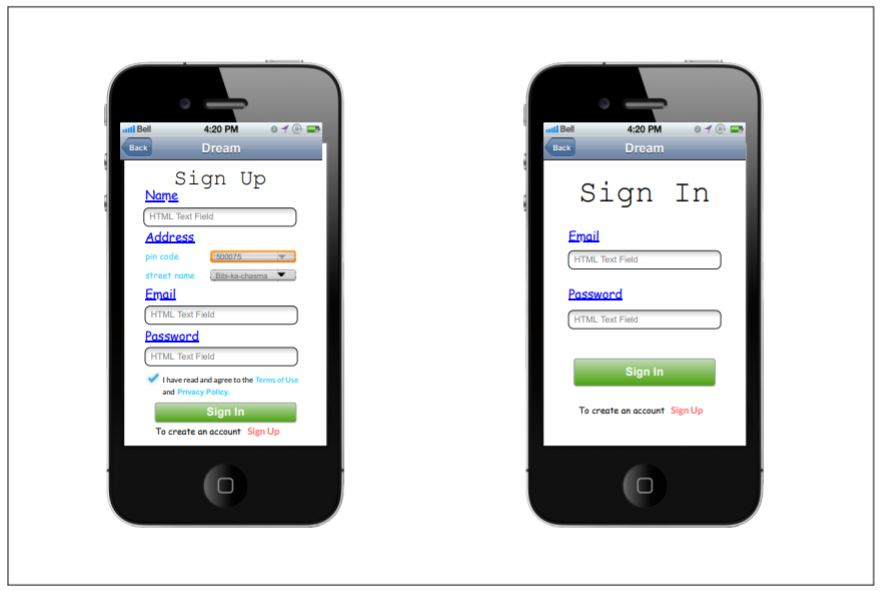
\includegraphics[page=1, width=\textwidth]{Images/sign_up_in.JPG}
	\caption{\label{fig:FE_image1}Sign Up, Sign In}
\end{figure}

\begin{figure}[H]
	\centering
    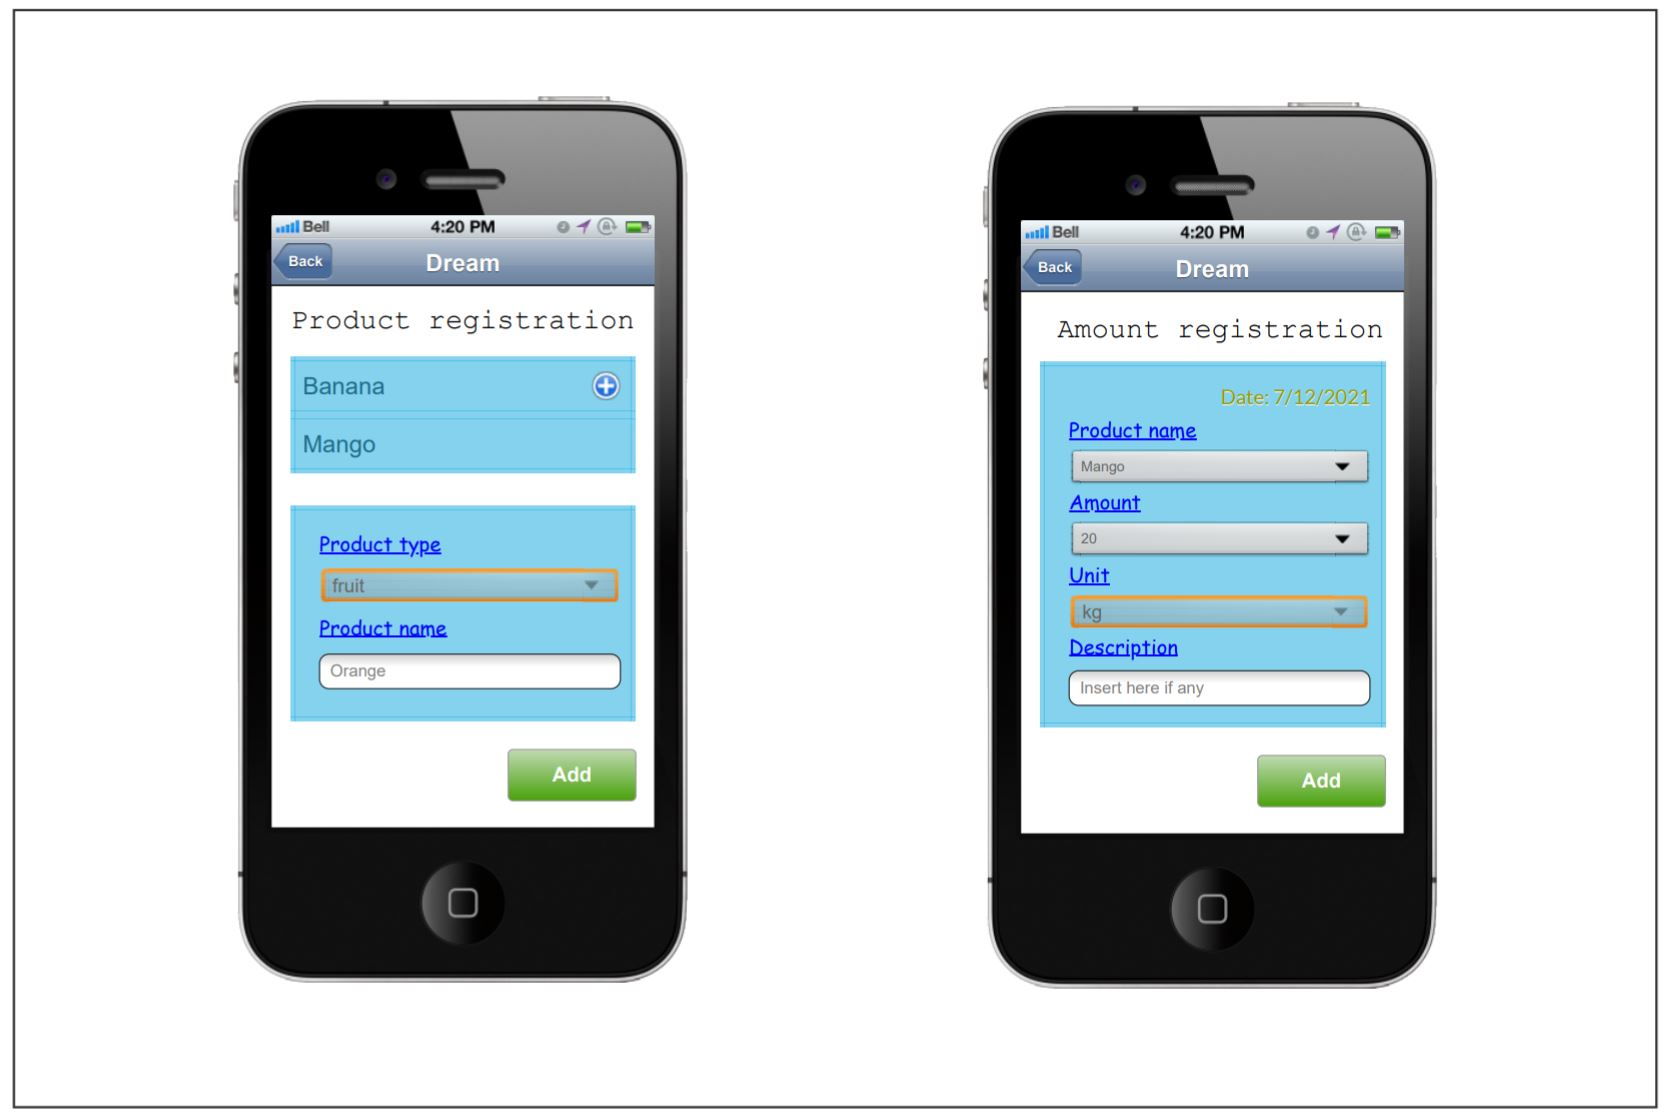
\includegraphics[page=1, width=\textwidth]{Images/product_amount_registration.JPG}
	\caption{\label{fig:FE_image2}Product registration, Amount registration}
\end{figure}



\begin{figure}[H]
	\centering
    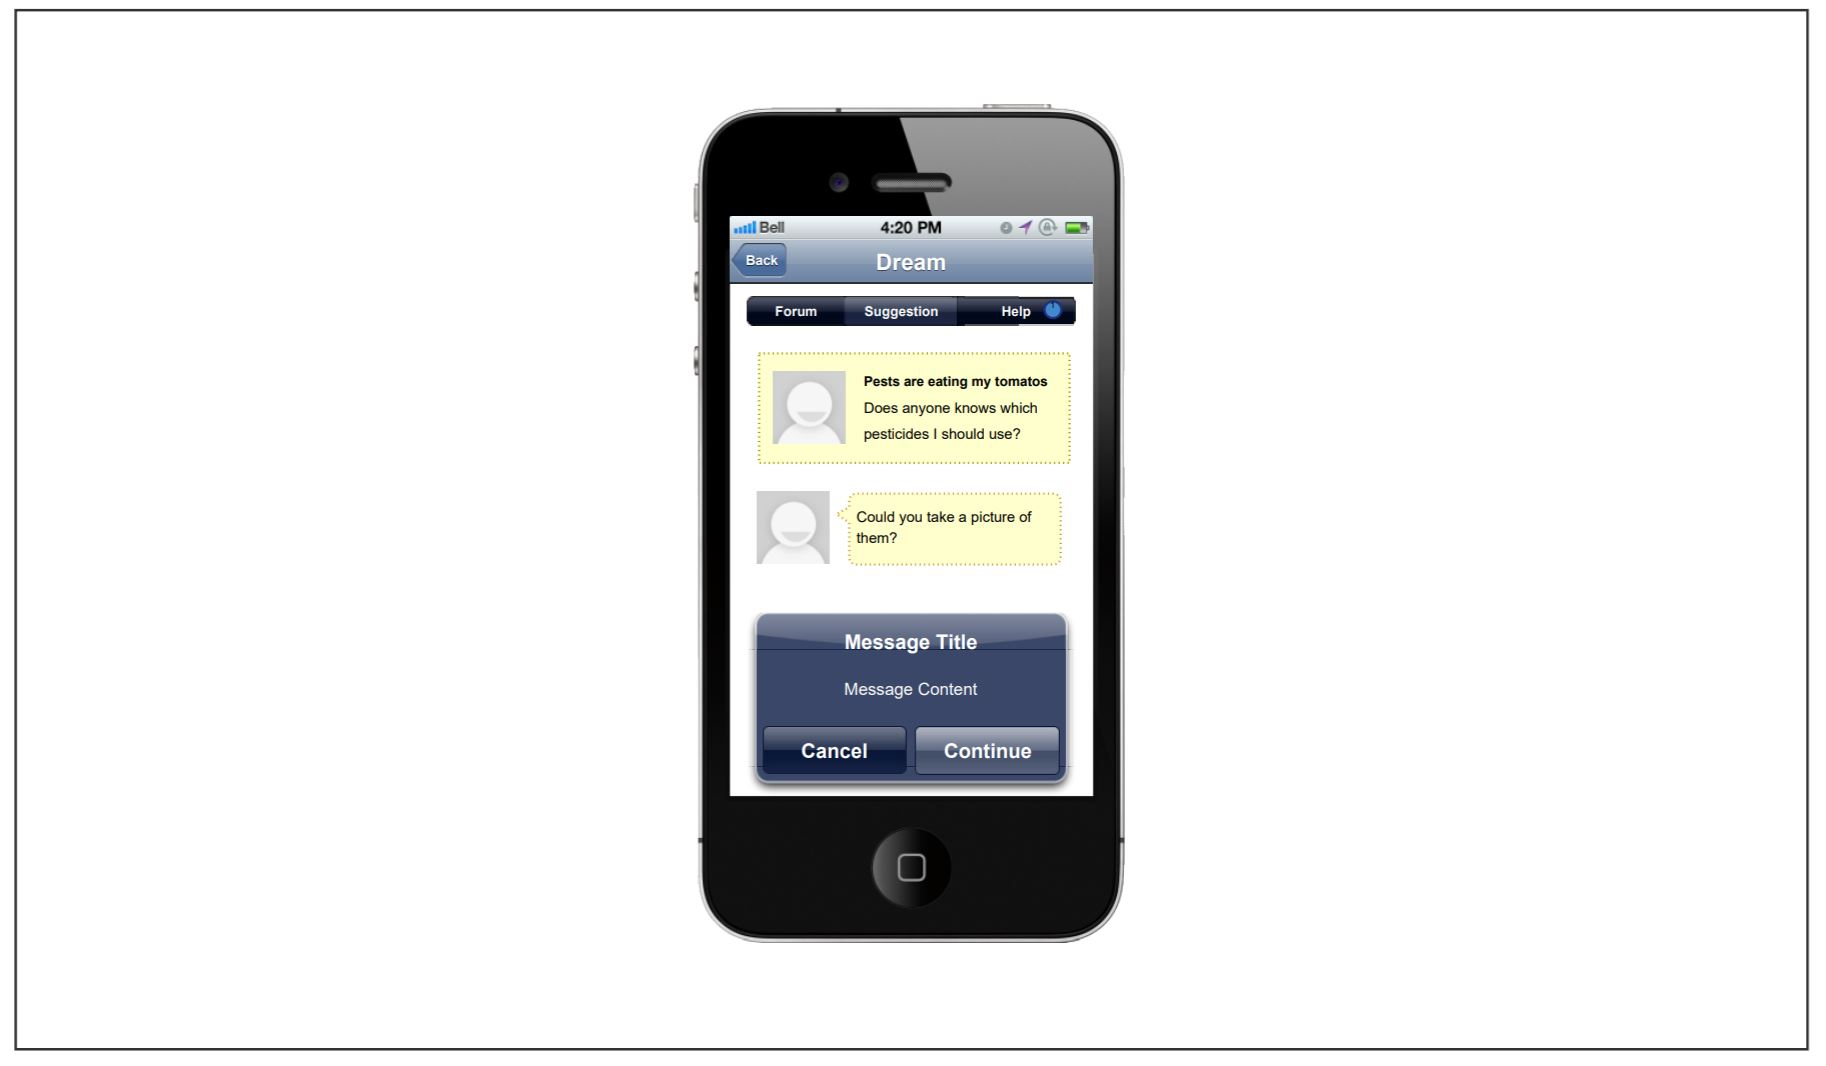
\includegraphics[page=1, width=\textwidth]{Images/message_insertion.JPG}
	\caption{\label{fig:FE_image3}Message insertion}
\end{figure}

\begin{figure}[H]
	\centering
    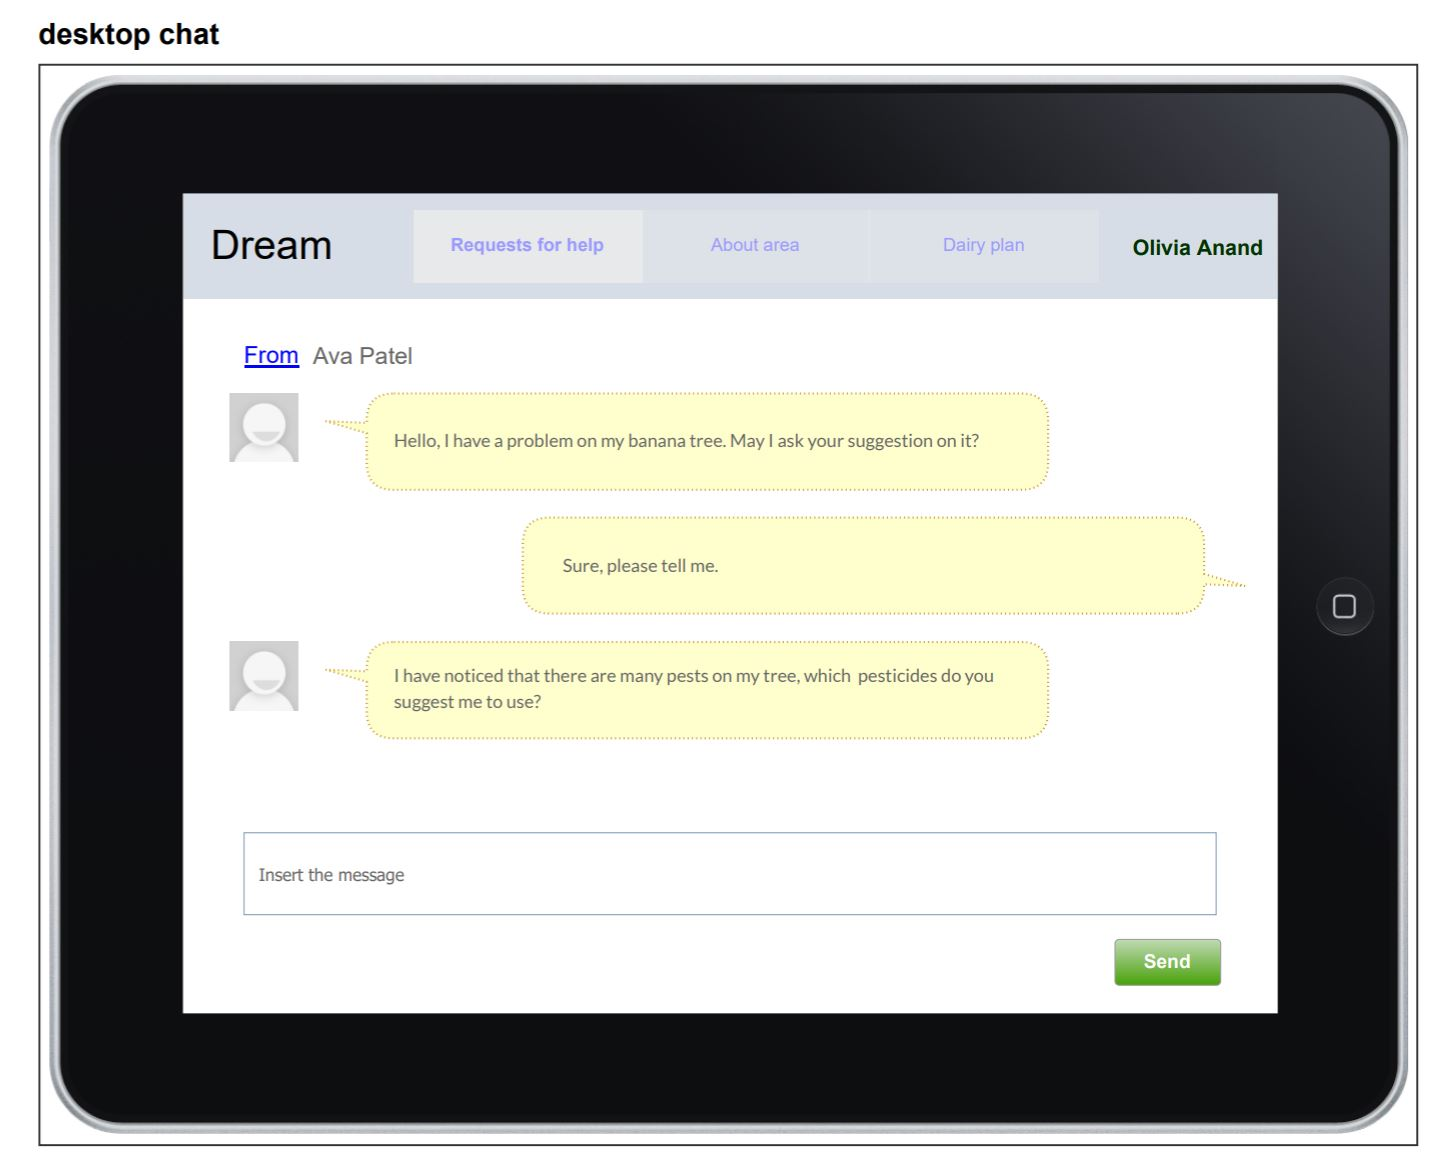
\includegraphics[page=1, width=\textwidth]{Images/desktop_chat.JPG}
	\caption{\label{fig:FE_image4}Desktop chat}
\end{figure}
\subsubsection{Hardware Interfaces}

\subsubsection{Software Interfaces}

\subsubsection{Communication Interfaces}


\subsection{Functional Requirements}
In this section we present the main \textbf{functional requirements} of the application while organizing them based on the actor that 

% #################### USE CASES TABLES ####################
\subsubsection{Users}
\label{sect:users_requirements}
% USE CASE TABLE 1: SIGN UP
 In this section there will be presented users use case tables \ldots
\begin{table}[H]
    \centering
    \begin{tabular}[c]{|l|p{0.75\textwidth}|}
        \hline % ---------------------------------------------------------------------
    	\textsc{id}                 &   U.1\\
    	\hline % ---------------------------------------------------------------------
    	\textsc{Name}               &   Sign up User with email\\
    	\hline % ---------------------------------------------------------------------
    	\textsc{Actor}             &   User\\
    	\hline % ---------------------------------------------------------------------
    	\textsc{Entry condition}   &   User has opened the Web page OR User has downloaded and opened the application on his smartphone\\
    	\hline % ---------------------------------------------------------------------
    	\textsc{Input}   &   Email to use for the registration\\
    	\hline % ---------------------------------------------------------------------
    	\textsc{Events flow}         &   %\footnotesize
            	                        \begin{itemize}
                                    	    \item The system displays the “Sign in” page
                                            \item User clicks on “Sign up”
                                            \item The system displays two fields: email and password
                                            \item User inserts the data and accepts the “Terms of services”
                                            \item User clicks on the “Confirm” button
                                            \item The system displays the acceptance of the registration and invites User to go to his inbox in order to confirm the registration
                                            \item User opens his inbox, checks the email and clicks on the confirmation link

                                        \end{itemize}\\
        \hline % ---------------------------------------------------------------------
        \textsc{Exit condition}    &  User registration has been successful: user data are stored in the system’s database. User can now login with his credentials\\
    	\hline % ---------------------------------------------------------------------
    	\textsc{Output}             &  \begin{itemize}
    	    \item User’s email is stored in the system’s database
            \item User receives the confirmation email

    	\end{itemize}\\
    	\hline % ---------------------------------------------------------------------
    	\textsc{Exceptions}         &  \begin{itemize}
    	    \item User inserts an email which is already stored in the database. So, after User clicks on “Confirm”, the system displays an error page which tells that User is already registered to the service and invites him to login with that email
            \item User inserts an invalid email. So, after User clicks on “Confirm”, the system displays the same sign up page with an error message, which suggests User to check the inserted email or to change it

    	\end{itemize}\\
    	\hline % ---------------------------------------------------------------------
        
    \end{tabular}
    \caption{\label{tab:user_sign_up}Sign up User}
\end{table}

\begin{figure}[H]
    \centering
    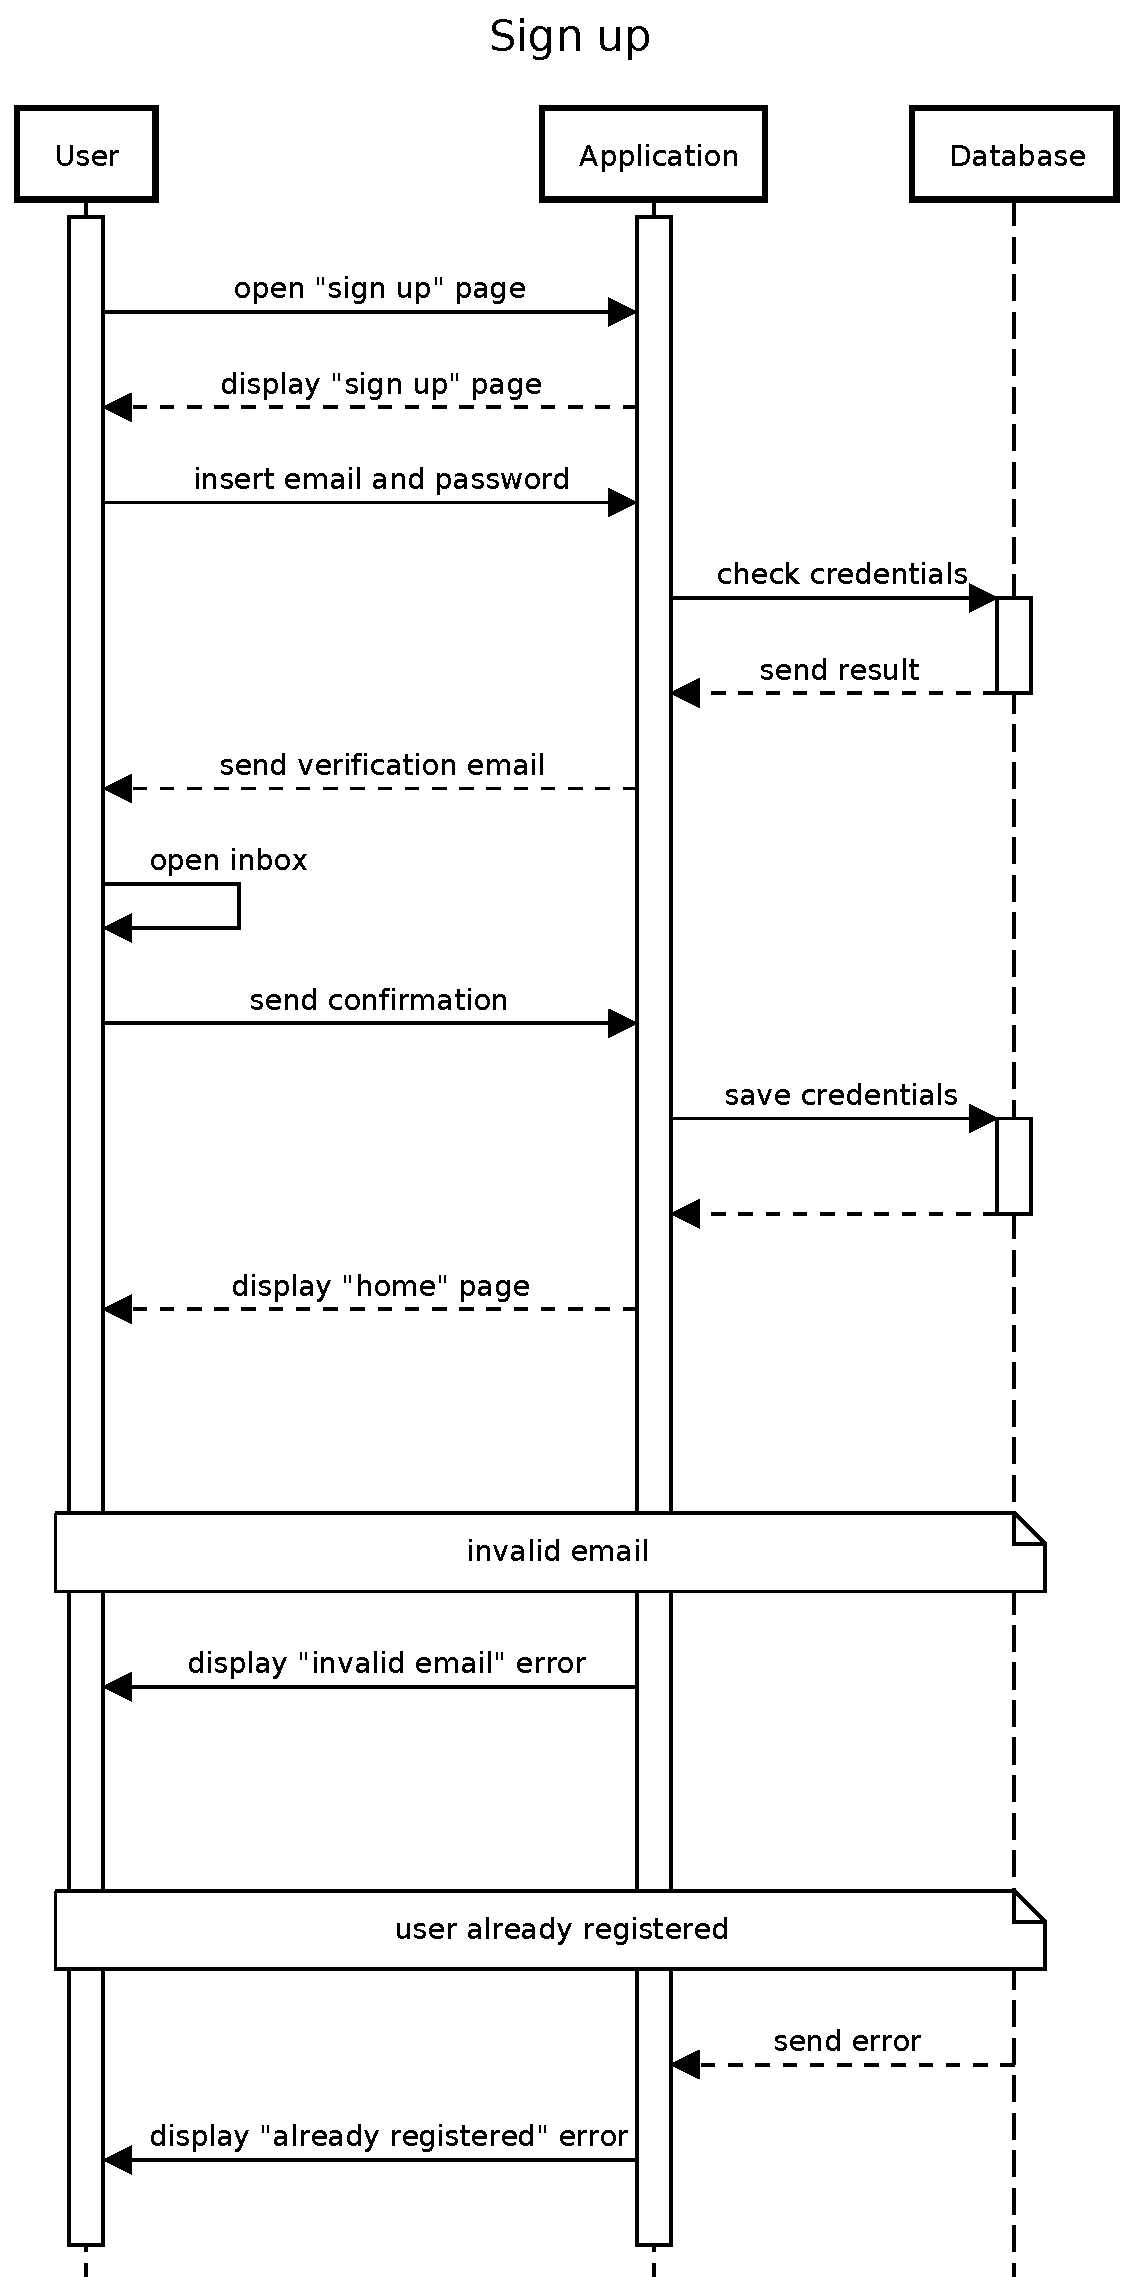
\includegraphics[scale=0.5]{Images/Sequence diagrams/User - sign up.pdf}

    \caption{Sign up User - sequence diagram}
    \label{fig:fig:seq_diag_sign_up}
\end{figure}

\begin{table}[H]
    \centering
    \begin{tabular}[c]{|l|p{0.75\textwidth}|}
        \hline % ---------------------------------------------------------------------
    	\textsc{id}                 &   U.2\\
    	\hline % ---------------------------------------------------------------------
    	\textsc{Name}               &   Login User\\
    	\hline % ---------------------------------------------------------------------
    	\textsc{Actor}             &   User\\
    	\hline % ---------------------------------------------------------------------
    	\textsc{Entry condition}   &   User has opened the Web page OR User has downloaded and opened the application on his smartphone\\
    	\hline % ---------------------------------------------------------------------
    	\textsc{Input}   &   User’s valid email and password\\
    	\hline % ---------------------------------------------------------------------
    	\textsc{Events flow}         &   %\footnotesize
            	                        \begin{itemize}
                                    	    \item The system displays the “Login” page
                                            \item User inserts his credentials (email, password) and clicks the “Login” button
                                            \item The system checks the correctness of the inserted credentials
                                            \item The system displays the home page


                                        \end{itemize}\\
        \hline % ---------------------------------------------------------------------
        \textsc{Exit condition}    &  User is logged in\\
    	\hline % ---------------------------------------------------------------------
    	\textsc{Output}             &  \begin{itemize}
    	    \item User inserts a wrong combination of email and password. The system displays the same page with an error message.

    	\end{itemize}\\
    	\hline % ---------------------------------------------------------------------
    	\textsc{Exceptions}         &  \begin{itemize}
    	    \item User inserts an email which is already stored in the database. So, after User clicks on “Confirm”, the system displays an error page which tells that User is already registered to the service and invites him to login with that email
            \item User inserts an invalid email. So, after User clicks on “Confirm”, the system displays the same sign up page with an error message, which suggests User to check the inserted email or to change it

    	\end{itemize}\\
    	\hline % ---------------------------------------------------------------------
        
    \end{tabular}

 

    
    \caption{\label{tab:user_login}Login User}
\end{table}

\begin{figure}[H]
    \centering
    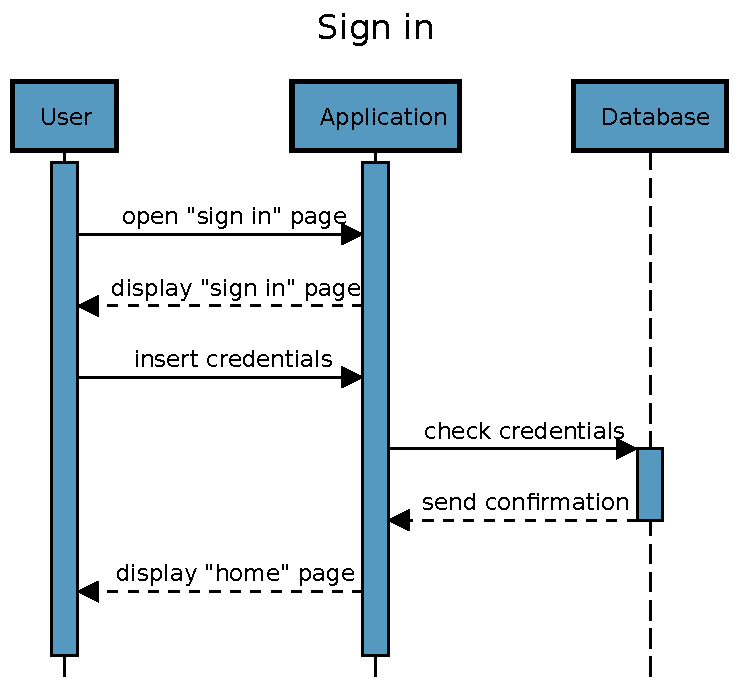
\includegraphics[scale=0.5]{Images/Sequence diagrams/User - sign in.pdf}

    \caption{Login User - sequence diagram}
    \label{fig:fig:seq_diag_sign_in}
\end{figure}



\subsubsection{Policy makers}
\label{sect:policy_maker_requirements}
% Moved to section 1.4 Definitions, acronyms, abbreviations


\begin{table}[H]
    \centering
    \begin{tabular}{|l|p{0.75\textwidth}|}
        \hline % ---------------------------------------------------------------------
    	\textsc{id}                 &   PM.1\\
    	\hline % ---------------------------------------------------------------------
    	\textsc{Name}               &   Visualize the performance data of each farmer\\
    	\hline % ---------------------------------------------------------------------
    	\textsc{Actor}             &   Policy maker\\
    	\hline % ---------------------------------------------------------------------
    	\textsc{Entry condition}   &   Policy maker has logged in\\
    	\hline % ---------------------------------------------------------------------
    	\textsc{Events flow}         &   %\footnotesize
            	                        \begin{itemize}
                                    	    \item Policy maker presses the button “Farmer’s performance”
                                    	    \item The system displays options to let user select filters about weather type, product type
                                    		\item Policy maker selects desired filters
                                    		\item The system displays the list of farmers divided by performance
                                    		\item Policy maker selects interested farmer’s name
                                    		\item The system shows detailed information about that farmer’s production
                                        \end{itemize}\\
        \hline % ---------------------------------------------------------------------
        \textsc{Exit condition}    &  The system returns to the main page of policy maker\\
    	\hline % ---------------------------------------------------------------------
    	\textsc{Output}             &  \begin{itemize}
    	    \item Policy maker has obtained the farmer's production data they were looking for
    	\end{itemize}\\
    	\hline % ---------------------------------------------------------------------
    	\textsc{Exception}         &  Policy maker could not find the name of farmer who should exist. The system displays the error message\\
    	\hline % ---------------------------------------------------------------------
        
    \end{tabular}
    \caption{\label{tab:visualize_farmer_performance}Visualize the performance data of farmers} 
\end{table}

\begin{figure}[H]
    \centering
    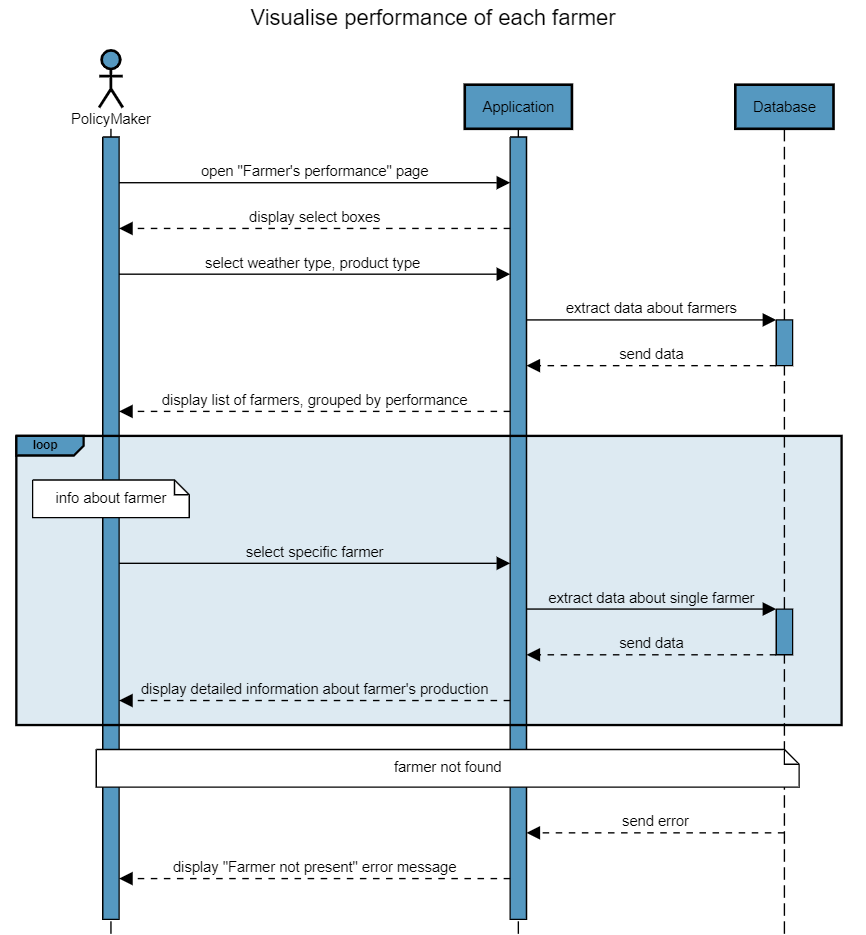
\includegraphics[scale=0.5]{Images/Sequence diagrams/SE2 - visualize performance (pm).png}
    \caption{Visualize the performance data of farmers - sequence diagram}
    \label{fig:my_label}
\end{figure}

\begin{table}[H]
    \centering
    \begin{tabular}{|l|p{0.75\textwidth}|}
        \hline % ---------------------------------------------------------------------
    	\textsc{id}                 &   PM.2\\
    	\hline % ---------------------------------------------------------------------
    	\textsc{Name}               &   Manage the incentives of high performing farmers \\
    	\hline % ---------------------------------------------------------------------
    	\textsc{Actor}             &   Policy maker\\
    	\hline % ---------------------------------------------------------------------
    	\textsc{Entry condition}   &   Policy maker has logged in\\
    	\hline % ---------------------------------------------------------------------
    	\textsc{Events flow}         &   %\footnotesize
            	                        \begin{itemize}
                                    	    \item Policy maker presses the button “Farmer’s performance”
                                    		\item The system displays a page with the list of farmers (grouped by performance) and a column which clarifies the status of their incentives 
                                       		\item Policy maker selects the interested farmer’s incentive column
                                    		\item The system shows detailed information about farmer’s incentives status
                                    		\item Policy maker clicks "Select incentive" button
                                    		\item The system shows the possible choices
                                    		\item Policy maker selects the incentive to give
                                    		\item The system shows the popup to ask a confirmation to proceed
                                    		\item Policy maker clicks "Confirm" button
                                    		\item The system shows the updated incentive column
                                        \end{itemize}\\
        \hline % ---------------------------------------------------------------------
        \textsc{Exit condition}    &  The system returns to the main page of policy maker\\
    	\hline % ---------------------------------------------------------------------
    	\textsc{Output}             &  \begin{itemize}
    	    \item Policy maker has managed the incentive to give
    	    \item The farmer correctly received the inventive
    	\end{itemize}\\
    	\hline % ---------------------------------------------------------------------
    	\textsc{Exception}         &  Policy maker wrongly selects an incentive data. The 
    	system shows a popup to ask a confirmation to proceed. The policy maker can redo the operation by clicking on “Cancel” button\\
    	\hline % ---------------------------------------------------------------------
        
    \end{tabular}
    \caption{\label{tab:visualize_incentives}Manage the incentives of farmers} 
\end{table}

\begin{figure}[H]
    \centering
    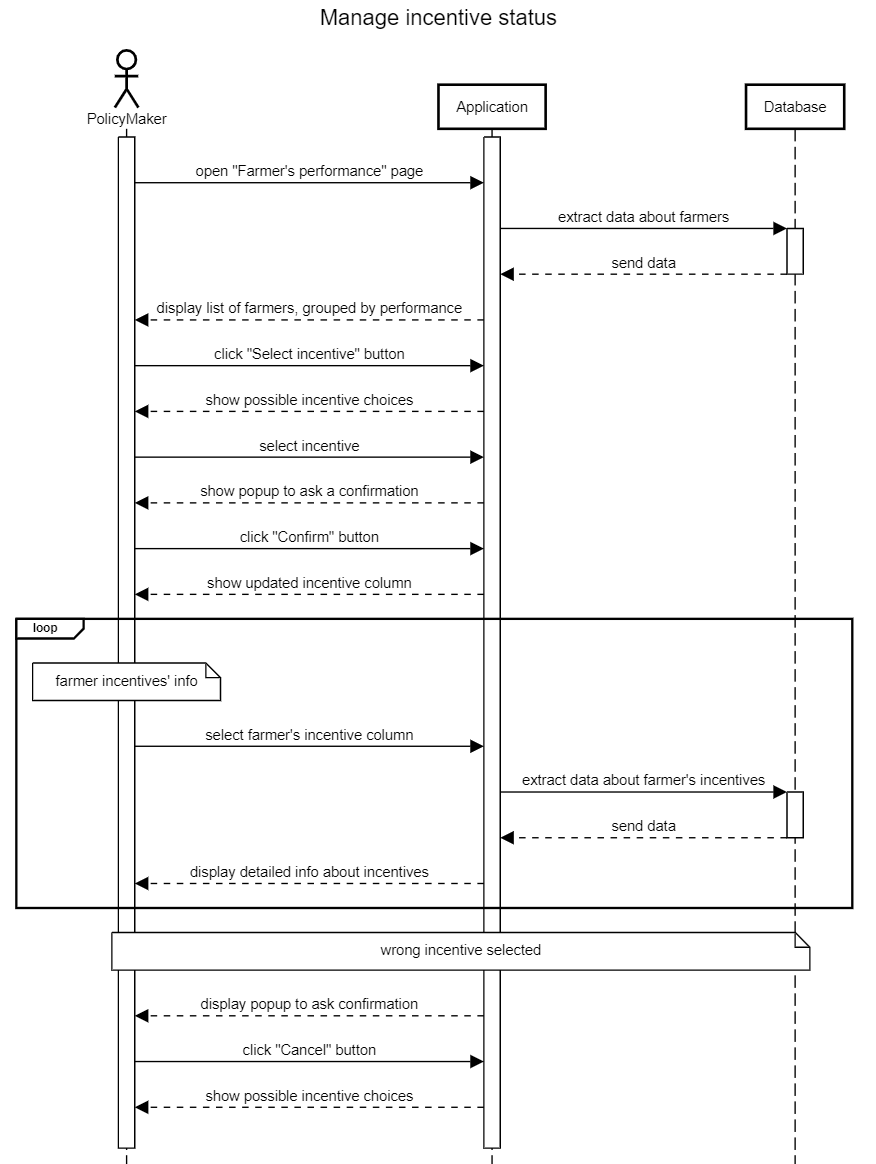
\includegraphics[scale=0.5]{Images/Sequence diagrams/SE2 - manage incentive status (pm).png}
    \caption{Manage the incentives of farmers - sequence diagram}
    \label{fig:my_label}
\end{figure}

\begin{table}[H]
    \centering
    \begin{tabular}{|l|p{0.75\textwidth}|}
        \hline % ---------------------------------------------------------------------
    	\textsc{id}                 &   PM.3\\
    	\hline % ---------------------------------------------------------------------
    	\textsc{Name}               &   Visualize the effectiveness of the steering initiatives\\
    	\hline % ---------------------------------------------------------------------
    	\textsc{Actor}             &   Policy maker\\
    	\hline % ---------------------------------------------------------------------
    	\textsc{Entry condition}   &   Policy maker has logged in\\
    	\hline % ---------------------------------------------------------------------
    	\textsc{Events flow}         &   %\footnotesize
            	                        \begin{itemize}
                                    	    \item Policy maker presses the button “Effectiveness of initiatives”
                                    	    \item The system displays options to let user select filters about weather type, product type
                                    		\item Policy maker selects the desired filters
                                    		\item The system displays a page with categorized farmers, highlighting those who have improved their performance significantly within a year
                                    		\item Policy maker selects interested farmer’s name
                                    		\item The system shows detailed information about the farmer’s performance trend, the problems encountered, the history of requests and visits
                                        \end{itemize}\\
        \hline % ---------------------------------------------------------------------
        \textsc{Exit conditions}    &  The system returns to the main page of policy maker\\
    	\hline % ---------------------------------------------------------------------
    	\textsc{Output}             &  \begin{itemize}
    	    \item Policy maker has obtained the history of performance data and interaction between farmers and agronomists they were looking for
    	\end{itemize}\\
    	\hline % ---------------------------------------------------------------------
    	\textsc{Exception}         &  Policy maker couldn’t find the name of farmer who should exist. The system displays the error message\\
    	\hline % ---------------------------------------------------------------------
        
    \end{tabular}
    \caption{\label{tab:visualize_iprovement}Visualize the effectiveness of the steering initiatives}
\end{table}

\begin{figure}[H]
    \centering
    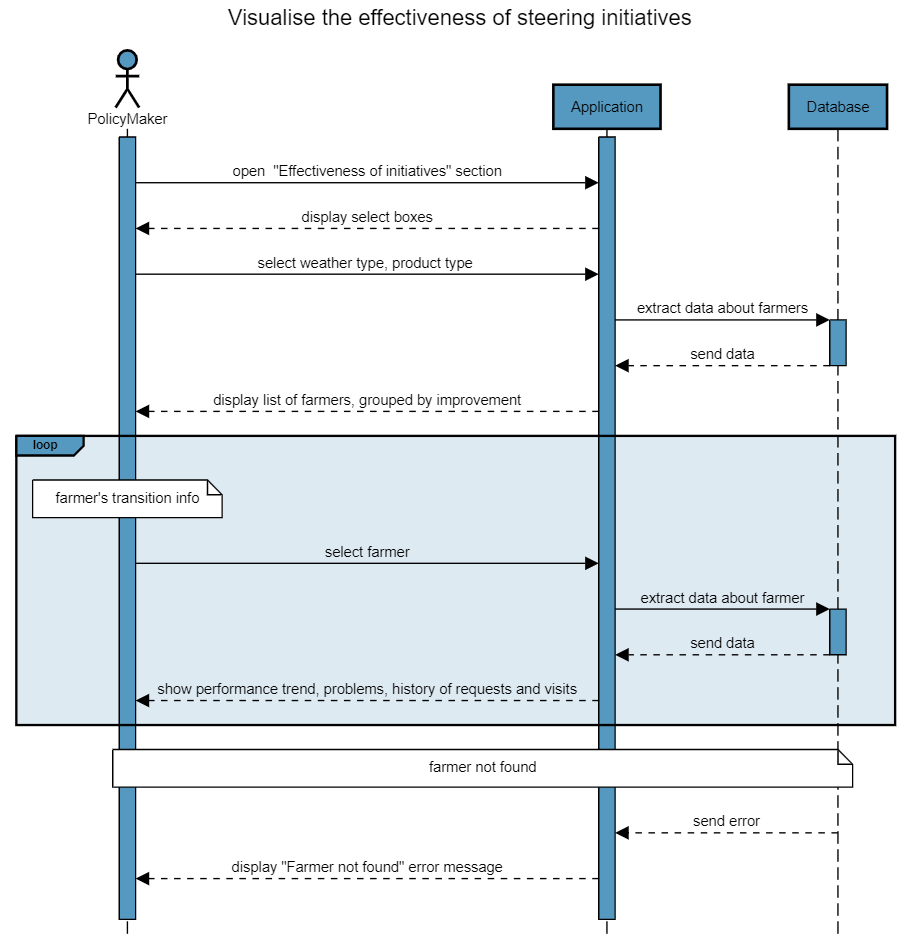
\includegraphics[scale=0.5]{Images/Sequence diagrams/SE2 - visualise effectiveness of steering initiatives (pm).png}
    \caption{Visualize the effectiveness of the steering initiatives - sequence diagram}
    \label{fig:my_label}
\end{figure}

\begin{table}[H]
    \centering
    \begin{tabular}{|l|p{0.75\textwidth}|}
        \hline % ---------------------------------------------------------------------
    	\textsc{id}                 &   PM.4\\
    	\hline % ---------------------------------------------------------------------
    	\textsc{Name}               &   Ask high performing farmers to write good practices\\
    	\hline % ---------------------------------------------------------------------
    	\textsc{Actor}             &   Policy maker\\
    	\hline % ---------------------------------------------------------------------
    	\textsc{Entry condition}   &   Policy maker has logged in\\
    	\hline % ---------------------------------------------------------------------
    	\textsc{Events flow}         &   %\footnotesize
            	                        \begin{itemize}
                                    	    \item Policy maker presses the button “Farmer’s performance”
                                    		\item The system displays a page with the list of farmers grouped by performance
                                    		\item Policy maker selects interested high performing farmer’s name
                                    		\item The system shows the detailed information about farmer’s production and "request writing" button
                                    		\item Policy maker clicks "equest writing" button
                                    		\item The system shows a popup to ask the confirmation to proceed
                                    		\item Policy maker clicks "Confirm" button
                                    		\item The system sends the request to the selected farmer and shows a message to notify the success of the operation
                                        \end{itemize}\\
        \hline % ---------------------------------------------------------------------
        \textsc{Exit condition}    &  The system returns to the Farmer’s performance page\\
    	\hline % ---------------------------------------------------------------------
    	\textsc{Output}             &  \begin{itemize}
    	    \item Policy maker has requested the high performing farmer to write their good practice
    	\end{itemize}\\
    	\hline % ---------------------------------------------------------------------
    	\textsc{Exception}         &  Policy maker wrongly selects a farmer. The 
    	system shows a popup to ask a confirmation to proceed. The policy maker can redo the operation by clicking on “Cancel” button\\
    	\hline % ---------------------------------------------------------------------
        
    \end{tabular}
    \caption{\label{tab:visualize_iprovement}Ask a farmer to write good practices} 
\end{table}

\begin{figure}[H]
    \centering
    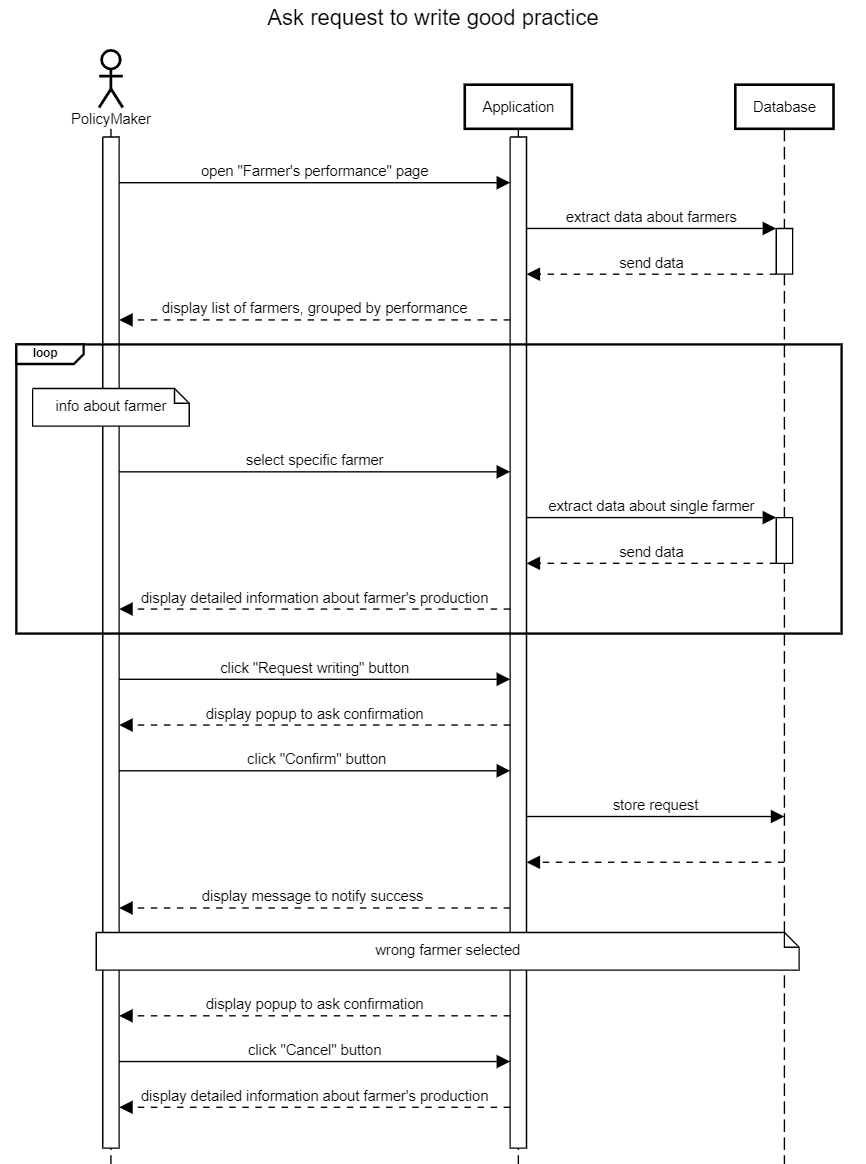
\includegraphics[scale=0.5]{Images/Sequence diagrams/SE2 - Ask request to write good practice (pm).png}
    \caption{Ask request to write good practice - sequence diagram}
    \label{fig:my_label}
\end{figure}


\subsubsection{Farmers}
\label{sect:farmer_requirements}
Synonims: system, application, service


% ####################### 1 PRODUCTION DATA UPLOAD ###################

\begin{table}[H]
    \centering
    \begin{tabular}[c]{|l|p{0.75\textwidth}|}
        \hline % ---------------------------------------------------------------------
    	\textsc{id}                 &   F.1\\
    	\hline % ---------------------------------------------------------------------
    	\textsc{Name}               &   Production data upload\\
    	\hline % ---------------------------------------------------------------------
    	\textsc{Actor}             &   Farmer\\
    	\hline % ---------------------------------------------------------------------
    	\textsc{Entry condition}   &   Farmer has logged in\\
    	\hline % ---------------------------------------------------------------------
    	\textsc{Events flow}         &   %\footnotesize
            	                        \begin{itemize}
                                    	    \item Farmer goes to the \textit{Record Production Data} section
                                    		\item The application displays a section that asks for \hyperref[tab:definitionsTable]{product information} and an \textit{Upload Button}
                                    		\item Farmer fills the mandatory fields of the current section and eventually the optional ones. Then press the \textit{Upload Button}.
                                    		\item The application displays a confirm popup revealing the summary of the information is going to be recorded, asking for Farmer confirmation through a \textit{Confirm Button}
                                    		\item The farmer confirms the submission by selecting the Confirm Button
                                        \end{itemize}\\
        \hline % ---------------------------------------------------------------------
        \textsc{Exit condition}    &  The application displays the summary page of both already uploaded product information and the previous submitted ones\\
    	\hline % ---------------------------------------------------------------------
    	\textsc{Output}             &  \begin{itemize}
    	    \item The system collects the new production data
    	    \item The farmer can visualize the list of both current production information and the previous ones
    	\end{itemize}\\
    	\hline % ---------------------------------------------------------------------
    	\textsc{Exception}         &  Farmer submits production data without filling the mandatory fields. In such case, the system displays an error message informing the Farmer about the missing field(s) required in order to achieve the goal\\
    	\hline % ---------------------------------------------------------------------
        
    \end{tabular}
    \caption{\label{tab:Production_data_submission}Production data upload}
\end{table}


\begin{figure}[H]
	\centering
    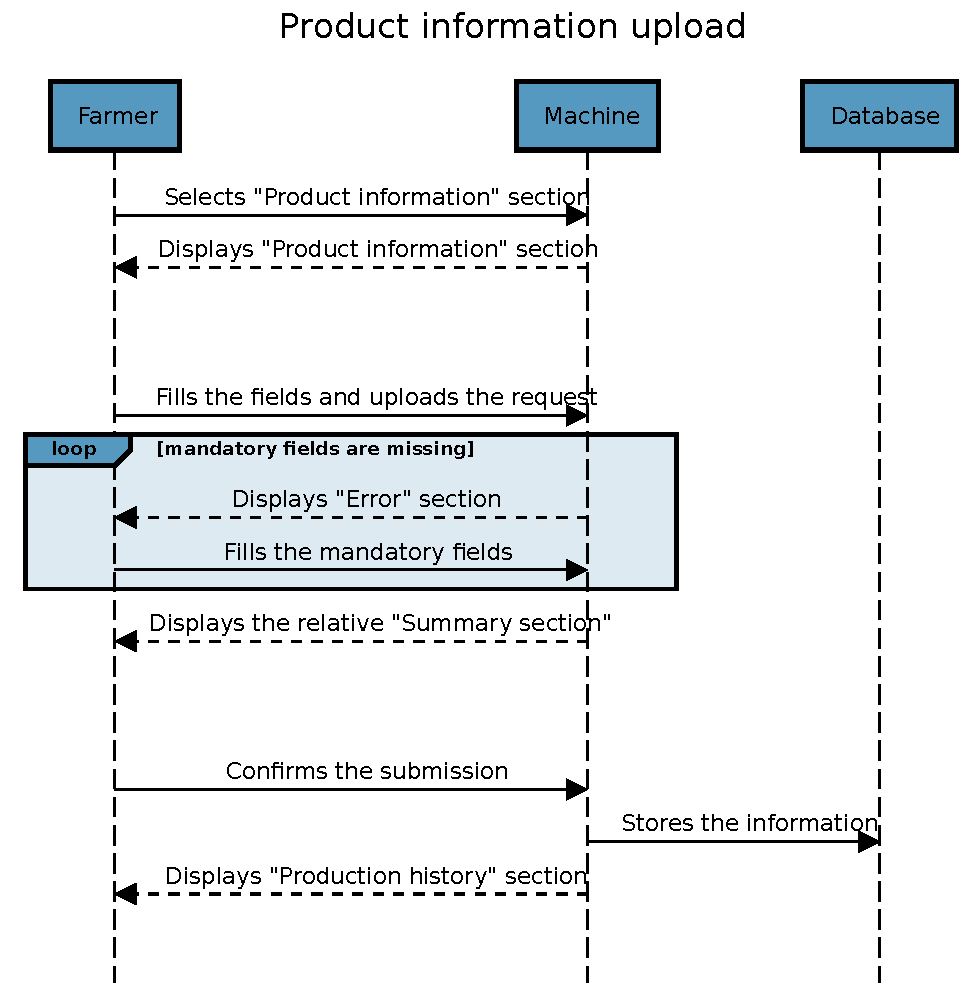
\includegraphics[page=1, width=\textwidth]{Images/SeqDiag/product_info_upload_seq_diag.pdf}
	\caption{\label{fig:product_info_seq_diag}Production data upload - sequence diagram}
\end{figure}


% ####################### 2 SUGGESTION REQUEST ###################

\begin{table}[H]
    \centering
    \begin{tabular}{|l|p{0.75\textwidth}|}
        \hline % ---------------------------------------------------------------------
    	\textsc{id}                 &   F.2\\
    	\hline % ---------------------------------------------------------------------
    	\textsc{Name}               &   Help/suggestion request\\
    	\hline % ---------------------------------------------------------------------
    	\textsc{Actor}             &   Farmer\\
    	\hline % ---------------------------------------------------------------------
    	\textsc{Entry condition}   &   Farmer has logged in\\
    	\hline % ---------------------------------------------------------------------
    	\textsc{Events flow}         &   %\footnotesize
            	                        \begin{itemize}
                                    	    \item Farmer selects the graphical section responsible of the private requests, called informally \textit{request section} for the sake of simplicity
                                    		\item The application displays a section that presents an eventual list of previous request chats and an additional button to send a new private request, called informally \textit{Send request element}
                                    		\item Farmer clicks on the send request button
                                    		\item The application displays a new section asking for the selection of the receivers
                                    		\item The farmer selects the contact he wants to send the request
                                    		\item The system displays a section with an editable text form, asks for the selection of the topic of the request and displays a send button
                                    		\item The farmer writes the request, fills the topic form and clicks on the send button
                                        \end{itemize}\\
        \hline % ---------------------------------------------------------------------
        \textsc{Exit condition}    &  The application displays the summary page of both already sent request chat and the previous submitted ones\\
    	\hline % ---------------------------------------------------------------------
    	\textsc{Output}             &  \begin{itemize}
    	    \item The system collects the new request chat
    	    \item The farmer can visualize the list of both current request chat and the previous ones
    	\end{itemize}\\
    	\hline % ---------------------------------------------------------------------
    	\textsc{Exception}         &  Farmer clicks on the request button without editing the text form. In such case, the system displays an error message informing the Farmer about the missing field required in order to achieve the goal\\
    	\hline % ---------------------------------------------------------------------
        
    \end{tabular}
    \caption{\label{tab:Help_request_submission}Help/suggestion request}

\end{table}

\begin{figure}[H]
	\centering
    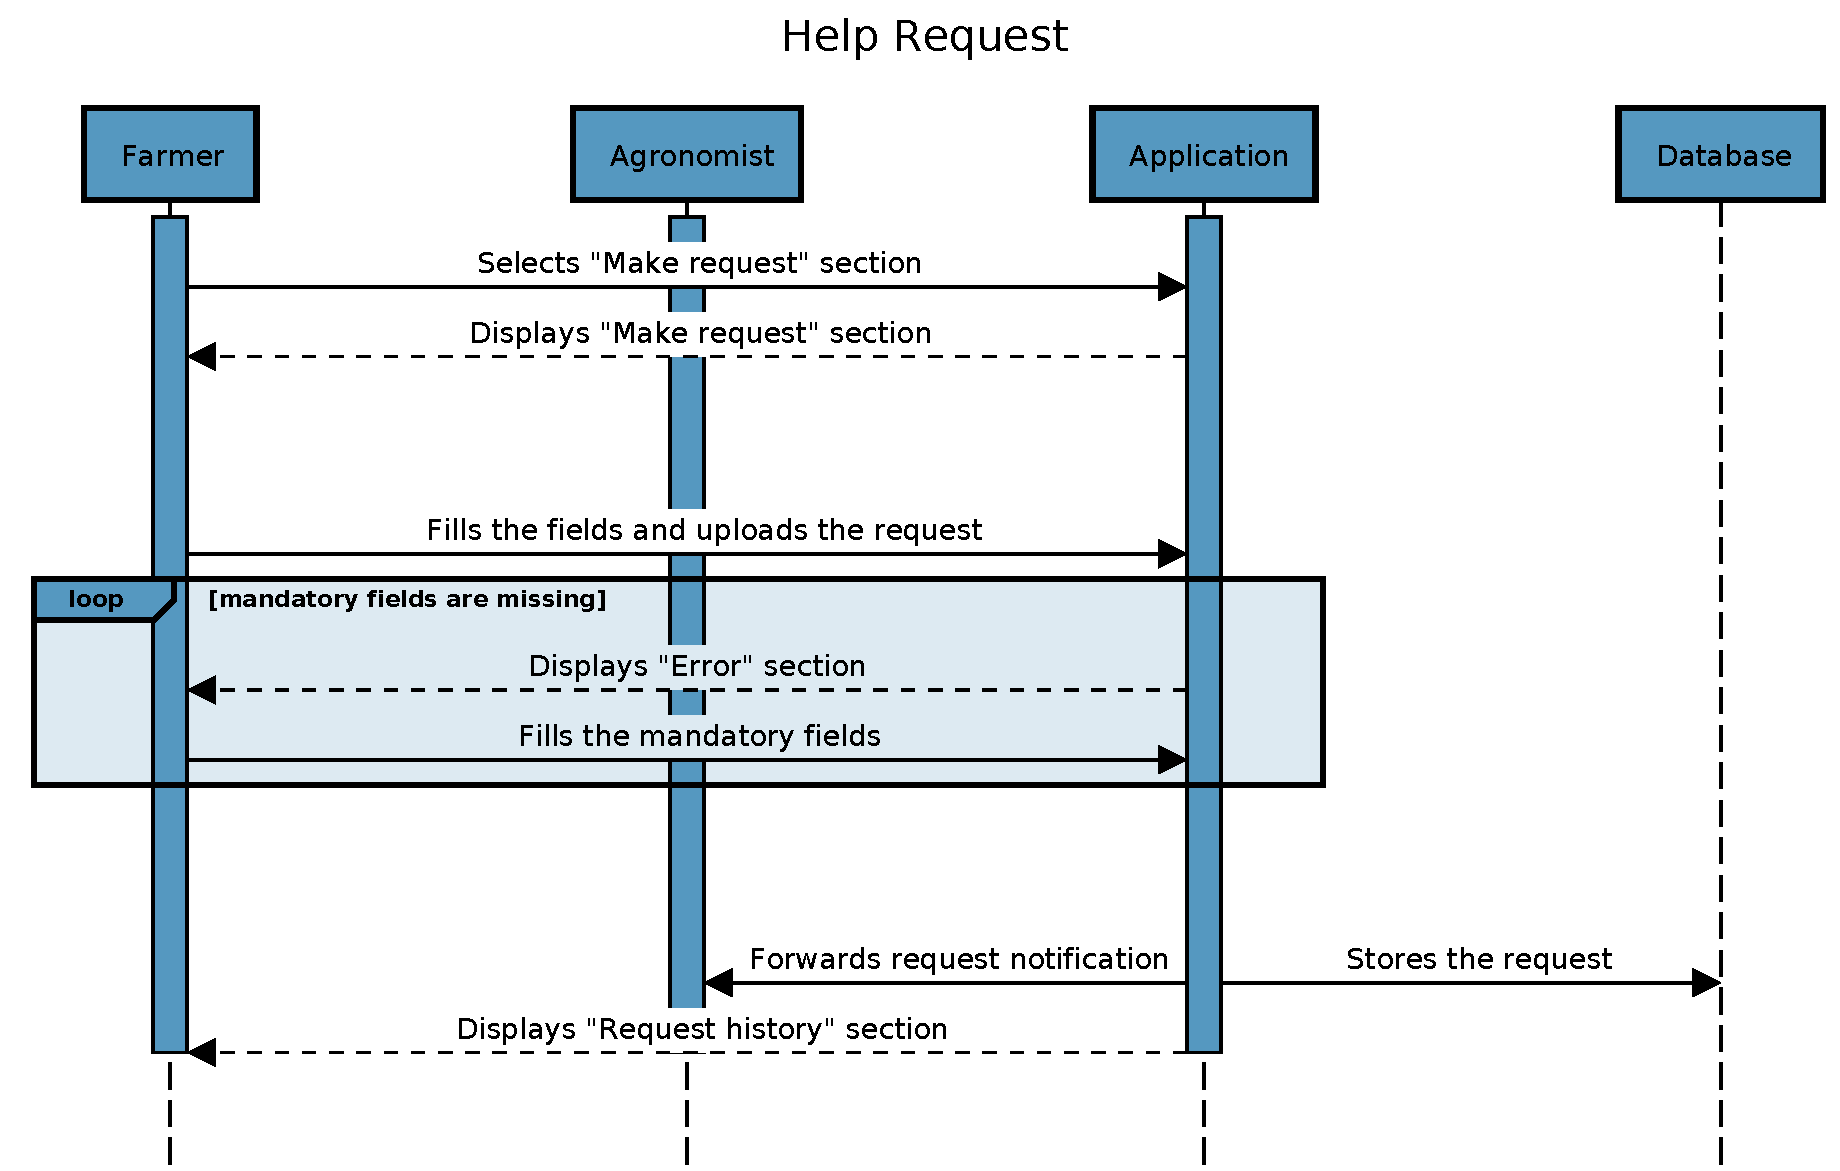
\includegraphics[page=1, width=\textwidth]{Images/SeqDiag/help_request_seq_diag.pdf}
	\caption{\label{fig:help_request_seq_diag}Help request - sequence diagram}
\end{figure}

% ####################### 3 FORUM GENERATION ###################

\begin{table}[H]
    \centering
    \begin{tabular}{|l|p{0.75\textwidth}|}
        \hline % ---------------------------------------------------------------------
    	\textsc{id}                 &   F.3\\
    	\hline % ---------------------------------------------------------------------
    	\textsc{Name}               &   Forum generation\\
    	\hline % ---------------------------------------------------------------------
    	\textsc{Actor}             &   Farmer\\
    	\hline % ---------------------------------------------------------------------
    	\textsc{Entry condition}   &   Farmer has logged in\\
    	\hline % ---------------------------------------------------------------------
    	\textsc{Events flow}         &   %\footnotesize
            	                        \begin{itemize}
                                    	    \item Farmer selects the graphical section responsible of the forum generation, called informally \textit{Forum section} for the sake of simplicity
                                    		\item The application displays a section that presents an eventual list that contains both previous submitted forums and the ones farmer replied, and an internal element to submit a new public forum, called informally \textit{forum upload button}
                                    		\item Farmer selects the forum upload button
                                    		\item The application displays a new section that present 3 mandatory fields (the topic/context of the thread, the title and the question content) and a submission button
                                    		\item The farmer fills all the mandatory fields and selects the submission button
                                    		\item The application displays a confirm popup revealing the summary of the information is going to be uploaded, asking for Farmer confirmation through a \textit{Confirm Button}
                                    		\item The farmer confirms the submission by selecting the Confirm Button
                                        \end{itemize}\\
        \hline % ---------------------------------------------------------------------
        \textsc{Exit condition}    &  The application displays the summary page containing both already submitted forum thread, the previous submitted ones and the ones to which the farmer replied\\
    	\hline % ---------------------------------------------------------------------
    	\textsc{Output}             &  \begin{itemize}
    	    \item The system collects the new forum thread
    	    \item The farmer can visualize the list containing both current forum thread, the previous submitted ones and the ones whose the farmer replied
    	\end{itemize}\\
    	\hline % ---------------------------------------------------------------------
    	\textsc{Exception}         &   Farmer submits Forum thread without filling all the mandatory fields. In such case, the system displays an error message informing the Farmer about the missing field(s) required in order to achieve the goal\\
    	\hline % ---------------------------------------------------------------------
        
    \end{tabular}


    \caption{\label{tab:Forum_generation}Forum generation}
\end{table}

\begin{figure}[H]
	\centering
    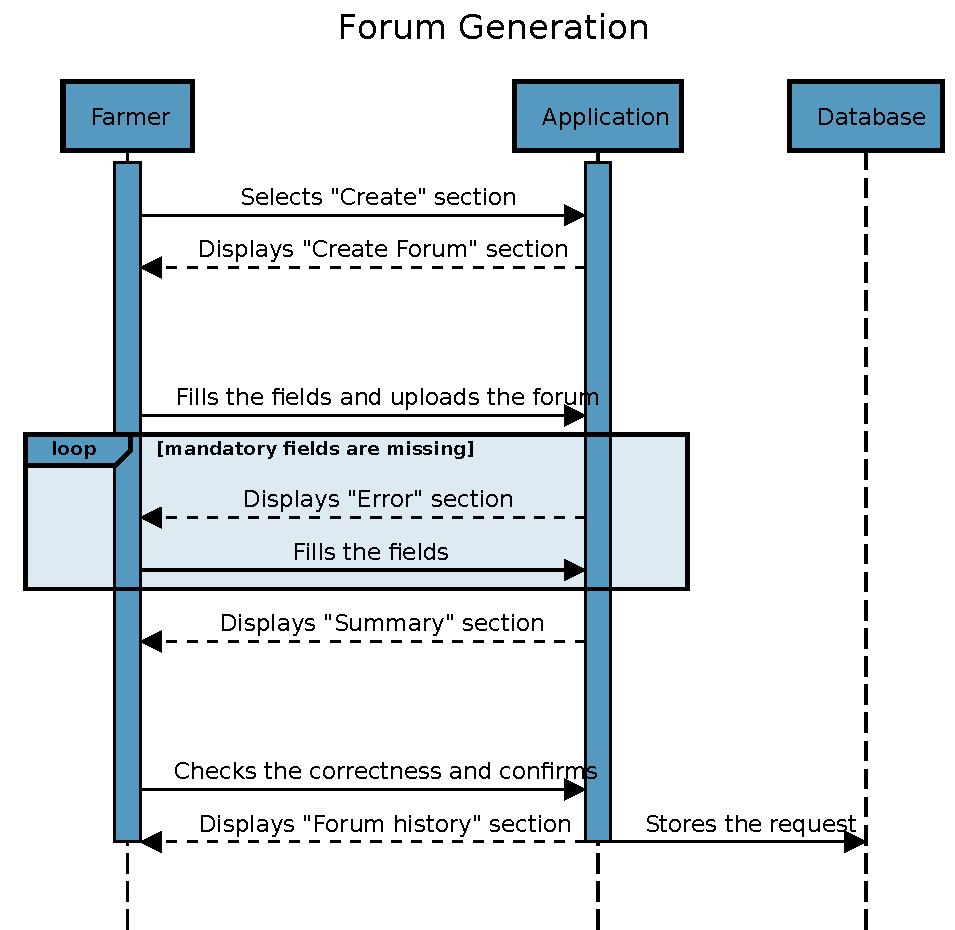
\includegraphics[page=1, width=\textwidth]{Images/SeqDiag/forum_generation_seq_diag.pdf}
	\caption{\label{fig:forum_generation_seq_diag}Forum generation - sequence diagram}
\end{figure}

% ####################### 4 PROBLEM INFORMATION ###################


\begin{table}[H]
    \centering
    \begin{tabular}{|l|p{0.75\textwidth}|}
        \hline % ---------------------------------------------------------------------
    	\textsc{id}                 &   F.4\\
    	\hline % ---------------------------------------------------------------------
    	\textsc{Name}               &   Problem information upload\\
    	\hline % ---------------------------------------------------------------------
    	\textsc{Actor}             &   Farmer\\
    	\hline % ---------------------------------------------------------------------
    	\textsc{Entry condition}   &   Farmer has logged in\\
    	\hline % ---------------------------------------------------------------------
    	\textsc{Events flow}         &   %\footnotesize
            	                        \begin{itemize}
                                    	    \item Farmer selects the graphical section responsible for the problem information submission, called informally \textit{Problems section}
                                    		\item The application displays a section that requires for information (described previously) and a "submit button"
                                    		\item Farmer fills the mandatory fields and eventually the optional ones, then selects the upload button
                                    		\item The application displays a confirm popup revealing the summary of the information is going to be uploaded, asking for Farmer confirmation through a \textit{Confirm Button}
                                    		\item The farmer confirms the submission by selecting the Confirm Button
                                        \end{itemize}\\
        \hline % ---------------------------------------------------------------------
        \textsc{Exit condition}    &  The application displays the summary page containing both already submitted problem information and the previous submitted ones\\
    	\hline % ---------------------------------------------------------------------
    	\textsc{Output}             &  \begin{itemize}
    	    \item The system collects the new problem information instance
    	    \item The farmer can visualize the list containing both the current submitted problem information and the previous submitted ones
    	\end{itemize}\\
    	\hline % ---------------------------------------------------------------------
    	\textsc{Exception}         &   Farmer submits problem information without filling all the mandatory fields. In such case, the system displays an error message informing the Farmer about the missing field(s) required in order to achieve the goal\\
    	\hline % ---------------------------------------------------------------------
        
    \end{tabular}

\caption{\label{tab:problem_information}Problem information upload}
\end{table}

\begin{figure}[H]
	\centering
    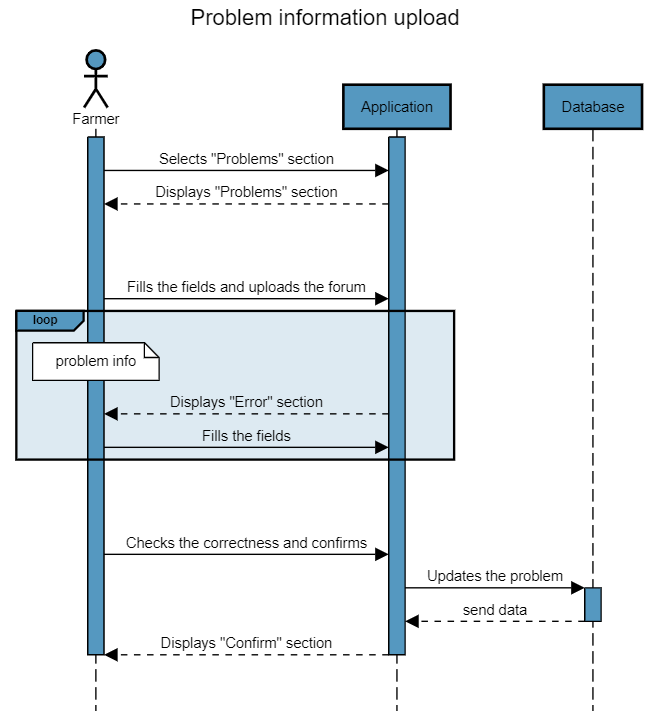
\includegraphics[page=1, width=\textwidth]{Images/Sequence diagrams/SW2- Problem information upload (fa).png}
	\caption{\label{fig:good_practice_seq_diag}Problem information upload - sequence diagram}
\end{figure}

% ####################### 5 GOOD PRACTICES ###################

\begin{table}[H]
    \centering
    \begin{tabular}{|l|p{0.75\textwidth}|}
        \hline % ---------------------------------------------------------------------
    	\textsc{id}                 &   F.5\\
    	\hline % ---------------------------------------------------------------------
    	\textsc{Name}               &   Good practices upload\\
    	\hline % ---------------------------------------------------------------------
    	\textsc{Actor}             &   Farmer\\
    	\hline % ---------------------------------------------------------------------
    	\textsc{Entry condition}   &   Farmer has logged in\\
    	\hline % ---------------------------------------------------------------------
    	\textsc{Events flow}         &   %\footnotesize
            	                        \begin{itemize}
                                    	    \item Farmer selects the graphical section responsible for the good practices document submission, called informally \textit{document section}
                                    		\item The application displays a section that requires for information (described previously) and a "submit button"
                                    		\item Farmer fills the mandatory fields and eventually the optional ones, then selects the upload button
                                    		\item The farmer confirms the submission by selecting the Confirm Button
                                        \end{itemize}\\
        \hline % ---------------------------------------------------------------------
        \textsc{Exit condition}    &  The application displays the summary page containing both already submitted document and the previous submitted ones\\
    	\hline % ---------------------------------------------------------------------
    	\textsc{Output}             &  \begin{itemize}
    	    \item The system collects the new document
    	    \item The farmer can visualize the list containing both the current submitted document and the previous submitted ones
    	\end{itemize}\\
    	\hline % ---------------------------------------------------------------------
    	\textsc{Exception}         &   Farmer submits document without filling all the mandatory fields. In such case, the system displays an error message informing the Farmer about the missing field(s) required in order to achieve the goal\\
    	\hline % ---------------------------------------------------------------------
        
    \end{tabular}

\caption{\label{tab:good_practice_submission}Good practices upload}
\end{table}

\begin{figure}[H]
	\centering
    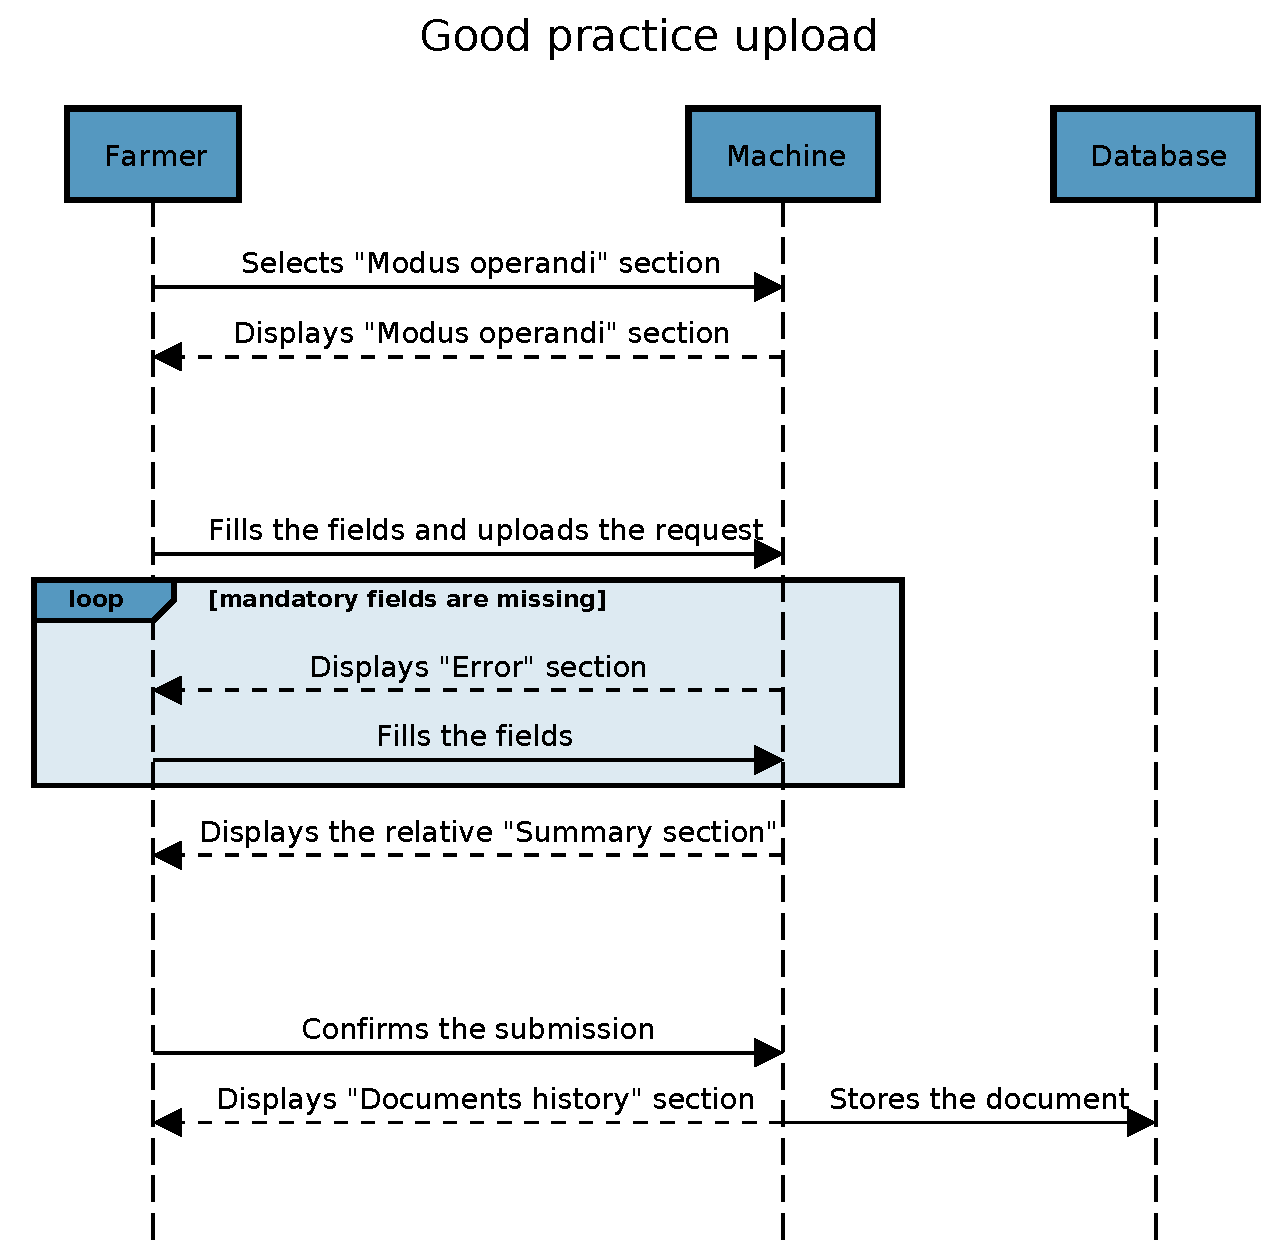
\includegraphics[page=1, width=\textwidth]{Images/SeqDiag/good_practice_seq_diag.pdf}
	\caption{\label{fig:good_practice_seq_diag}Good practices upload - sequence diagram}
\end{figure}


\begin{table}[H]
    \centering
    \begin{tabular}{|l|p{0.75\textwidth}|}
        \hline % ---------------------------------------------------------------------
    	\textsc{id}                 &   F.6\\
    	\hline % ---------------------------------------------------------------------
    	\textsc{Name}               &   Visualize relevant data\\
    	\hline % ---------------------------------------------------------------------
    	\textsc{Actor}             &   Farmer\\
    	\hline % ---------------------------------------------------------------------
    	\textsc{Entry condition}   &   Farmer has logged in\\
    	\hline % ---------------------------------------------------------------------
    	\textsc{Events flow}         &   %\footnotesize
            	                        \begin{itemize}
                                    	    \item Farmer selects the graphical section responsible for the relevant data visualization, called informally \textit{Relevant data section}
                                        \end{itemize}\\
        \hline % ---------------------------------------------------------------------
        \textsc{Exit condition}    &  The application displays a section containing information about weather forecasts, farm related tools suggestion, agronomist visit time, amount of water used that month, soil humidity etc.)\\
    	\hline % ---------------------------------------------------------------------
    	\textsc{Output}             &  \begin{itemize}
    	    \item The farmer can visualize relevant information
    	    \item Farmer can interact with information (links to shop websites etc.)
    	\end{itemize}\\
    	\hline % ---------------------------------------------------------------------
    	\textsc{Exception}         &   If the internet connection is lost, the application displays a section informing the task cannot be achieved\\
    	\hline % ---------------------------------------------------------------------
        
    \end{tabular}

\caption{\label{tab:visualize_relevant_data}Visualize relevant data for farmers}
\end{table}

\begin{figure}[H]
	\centering
    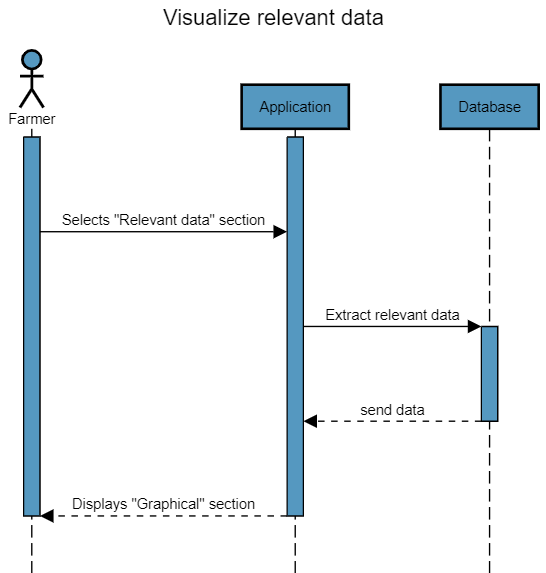
\includegraphics[page=1, width=\textwidth]{Images/Sequence diagrams/SW2 - Visualize relevant data (fa).png}
	\caption{\label{fig:good_practice_seq_diag} Visualize relevant data - sequence diagram}
\end{figure}

\subsubsection{Agronomists}
\label{sect:agronomist_requirements}
In this section there will be presented agronomists use case tables \ldots

% USE CASE TABLE 1: INSERT THE AREA AGRONOMISTS ARE RESPONSIBLE OF
\begin{table}[H]
    \centering
    \begin{tabular}[c]{|l|p{0.75\textwidth}|}
        \hline % ---------------------------------------------------------------------
    	\textsc{id}                 &   A.1\\
    	\hline % ---------------------------------------------------------------------

    	\textsc{Name}               &   Add an area under the agronomist's responsibility\\
    	\hline % ---------------------------------------------------------------------
    	\textsc{Actor}             &   Agronomist\\
    	\hline % ---------------------------------------------------------------------
    	\textsc{Entry condition}   &   Agronomist has logged in\\
    	\hline % ---------------------------------------------------------------------
    	\textsc{Events flow}         &   %\footnotesize
            	                        \begin{itemize}
                                    	    \item Agronomist goes to the "Area management" section
                                    	    \item The system extracts the data from the database and displays the list of areas under the agronomist's responsibility
                                    	    \item Agronomist presses the button “Add an area”
                                    		\item The system displays a page with all the available areas and a search bar
                                    		\item Agronomist makes a research based on the name/location of the area
                                    		\item The system shows the results
                                    		\item Agronomist selects the desired area
                                    		\item The system shows the details of the area selected (number of farmers, number of agronomists, weather information, etc)
                                    		\item Agronomist clicks on “Add this area”
                                    		\item The system updates the database and shows a message of insertion completed
                                        \end{itemize}\\
        \hline % ---------------------------------------------------------------------
        \textsc{Exit condition}    &  The system displays the "Area management" section\\
    	\hline % ---------------------------------------------------------------------
    	\textsc{Output}             &  \begin{itemize}
    	    \item The system has added the agronomist in the database as responsible for that area
    	\end{itemize}\\
    	\hline % ---------------------------------------------------------------------
    	\textsc{Exception}         &  Agronomist wrongly clicks “Add this area”. The system displays a popup notifying that he will be added as responsible for that area and the agronomist clicks on “Cancel” button\\
    	\hline % ---------------------------------------------------------------------
        
    \end{tabular}
    \caption{\label{tab:responsible_area_insertion}Add an area for an agronomist}
\end{table}

\begin{figure}[H]
    \centering
    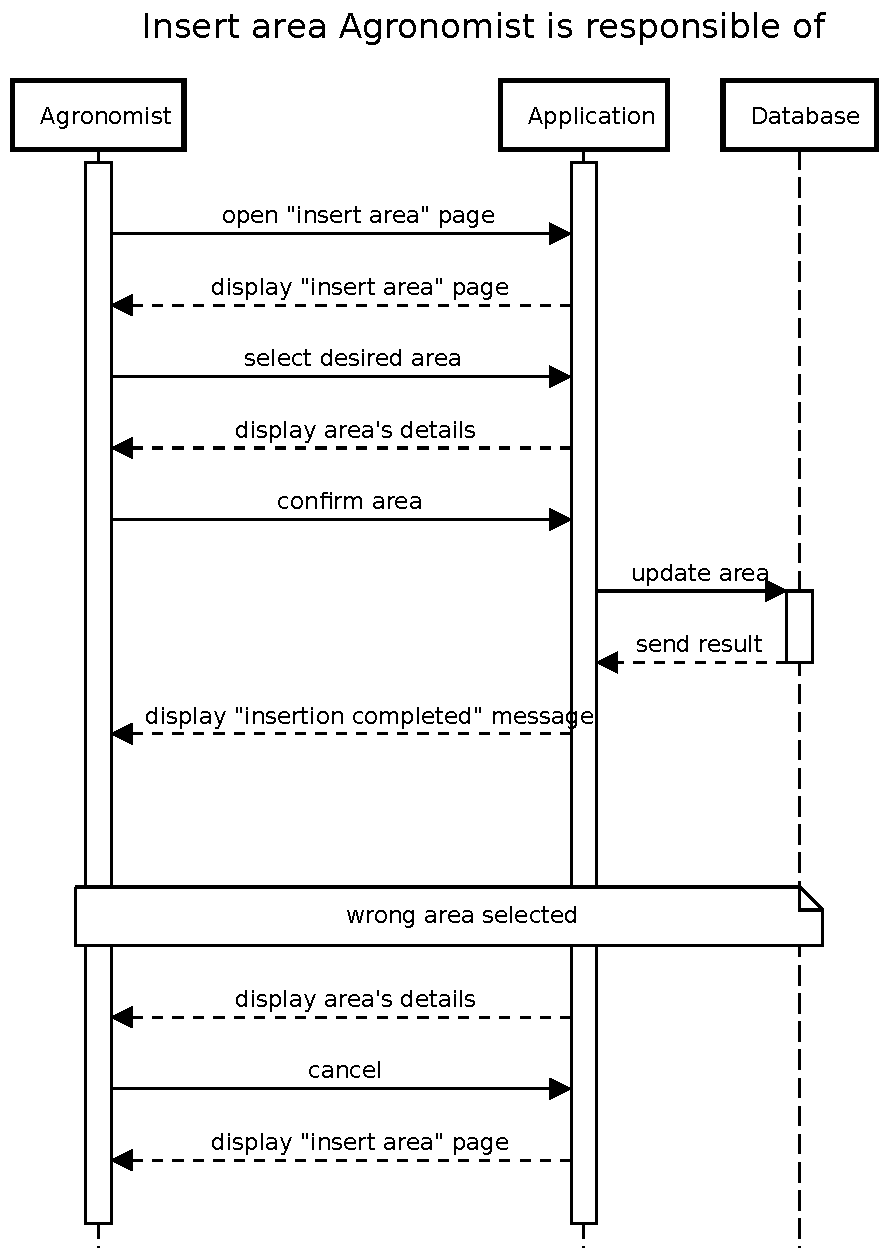
\includegraphics[scale=0.75]{Images/Sequence diagrams/Agronomist - Insert area.pdf}

    \caption{Add an area for an agronomist - sequence diagram}
    \label{fig:fig:seq_diag_insert_area}

    
\end{figure}


% USE CASE 2: REMOVING AN AREA UNDER THE AGRONOMIST'S RESPONSIBILITY
\begin{table}[H]
    \centering
    \begin{tabular}[c]{|l|p{0.75\textwidth}|}
        \hline % ---------------------------------------------------------------------
    	\textsc{id}                 &   A.2\\
    	\hline % ---------------------------------------------------------------------
    	\textsc{Name}               &   Remove an area under the agronomist's responsibility\\
    	\hline % ---------------------------------------------------------------------
    	\textsc{Actor}             &   Agronomist\\
    	\hline % ---------------------------------------------------------------------
    	\textsc{Entry conditions}   &  
    	\begin{itemize}
                                    	    \item Agronomist has logged in
                                    	    \item Agronomist is responsible for at least one area
                                        \end{itemize}\\
    	\hline % ---------------------------------------------------------------------
    	\textsc{Events flow}         &   %\footnotesize
            	                        \begin{itemize}
                                    	    \item Agronomist goes to the "Area management" section
                                    	    \item The system extracts the data from the database and displays the list of areas under the agronomist's responsibility
                                    	    \item Agronomist presses the button “Remove this area” next to the desired area
                                    		\item The system displays a popup asking for confirmation
                                    		\item Agronomist clicks on “Confirm”
                                    		\item The system updates the database and shows a message of removal completed
                                        \end{itemize}\\
        \hline % ---------------------------------------------------------------------
        \textsc{Exit condition}    &  The system displays the "Area management" section\\
    	\hline % ---------------------------------------------------------------------
    	\textsc{Output}             &  \begin{itemize}
    	    \item The system has removed the agronomist in the database as responsible for that area
    	\end{itemize}\\
    	\hline % ---------------------------------------------------------------------
    	\textsc{Exception}         &  Agronomist wrongly clicks “Remove this area”. The system displays a popup notifying that he will be removed as responsible for that area and the agronomist clicks on “Cancel” button\\
    	\hline % ---------------------------------------------------------------------
        
    \end{tabular}
    \caption{\label{tab:responsible_area_insertion}Remove an area for an agronomist}
\end{table}

% USE CASE TABLE 2: ACCESS THE "REQUEST FOR HELP" SECTION

\begin{table}[H]
    \centering
    \begin{tabular}[c]{|l|p{0.75\textwidth}|}
        \hline % ---------------------------------------------------------------------
    	\textsc{id}                 &   A.3\\
    	\hline % ---------------------------------------------------------------------
    	\textsc{Name}               &   Visualize and answer to requests for help\\
    	\hline % ---------------------------------------------------------------------
    	\textsc{Actor}             &   Agronomist\\
    	\hline % ---------------------------------------------------------------------
    	\textsc{Entry condition}   &   Agronomist has logged in\\
    	\hline % ---------------------------------------------------------------------
    	\textsc{Events flow}         &   %\footnotesize
            	                        \begin{itemize}
                                    	    \item Agronomist goes to the “Requests for help” section
                                    		\item The system extracts the data from the database and displays a search bar and the list of conversations (sorted by recent activity), marking the ones which contains new messages
                                    		\item Agronomist selects a conversation
                                    		\item The system displays all the messages contained in that conversation and a text box
                                    		\item Agronomist writes in the text box an answer to the request and clicks “Send”
                                    		\item The system adds the message to the database
                                        \end{itemize}\\
        \hline % ---------------------------------------------------------------------
        \textsc{Exit condition}    &  The system remains in the same page, refreshing its content\\
    	\hline % ---------------------------------------------------------------------
    	\textsc{Output}             &  \begin{itemize}
    	    \item The system adds the message to the database
    	    \item The system notifies the participants of that conversation about the new message
    	\end{itemize}\\
    	\hline % ---------------------------------------------------------------------
    	\textsc{Exception}         &  The system cannot connect to the database/server. The system displays an error message.\\
    	\hline % ---------------------------------------------------------------------
        
    \end{tabular}
    \caption{\label{tab:help_request_section_access}Visualize and answer to requests for help}
\end{table}

\begin{figure}[H]
    \centering
    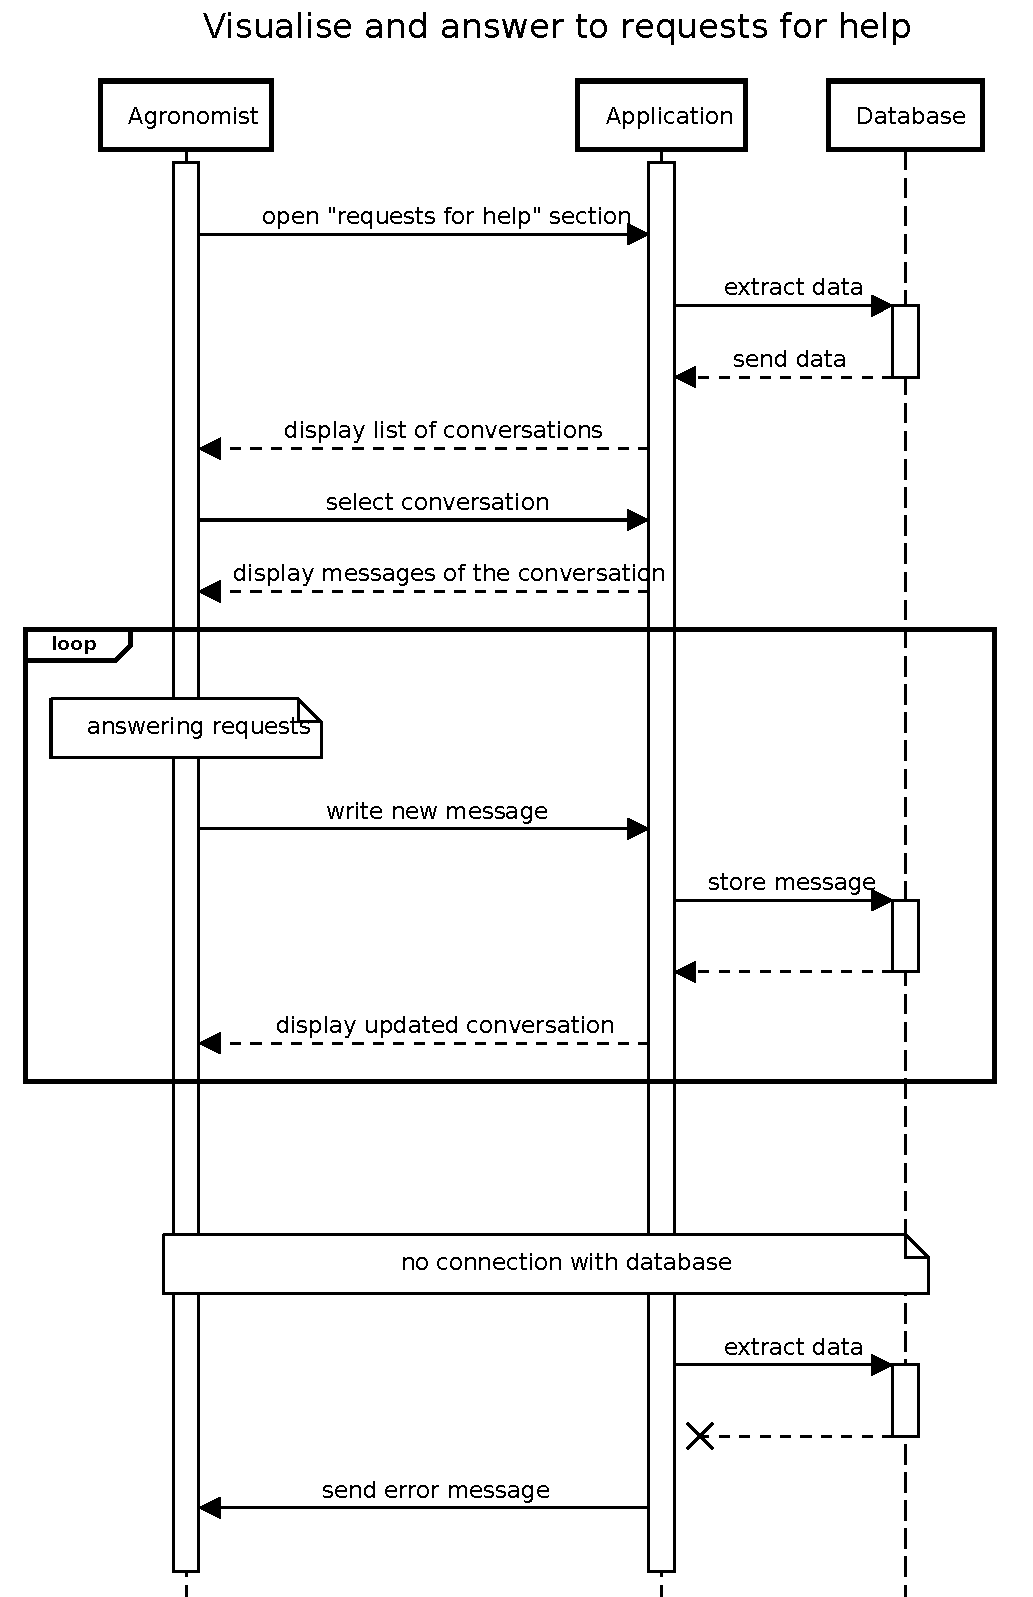
\includegraphics[scale=0.75]{Images/Sequence diagrams/Agronomist - visualise and answer requests for help.pdf}

    \caption{Visualize and answer to requests for help - sequence diagram}
    \label{fig:fig:seq_diag_answer_request}
\end{figure}

% USE CASE TABLE 3: VISUALIZE DATA OF THE AREA

\begin{table}[H]
    \centering
    \begin{tabular}[c]{|l|p{0.75\textwidth}|}
        \hline % ---------------------------------------------------------------------
    	\textsc{id}                 &   A.4\\
    	\hline % ---------------------------------------------------------------------
    	\textsc{Name}               &   Visualize data of an area\\
    	\hline % ---------------------------------------------------------------------
    	\textsc{Actor}             &   Agronomist\\
    	\hline % ---------------------------------------------------------------------
    	\textsc{Entry condition}   &   Agronomist has logged in\\
    	\hline % ---------------------------------------------------------------------
    	\textsc{Events flow}         &   %\footnotesize
            	                        \begin{itemize}

                                    	    \item Agronomist goes to the “Information about areas” section
                                    	    \item The system extract the data from the database and displays the list of areas under the agronomist's responsibility
                                    	    \item Agronomist selects an area
                                    		\item The system displays a page with three main options: “Weather forecasts”, “Farmers’ performing situation” and "Problems encountered"
                                    		\item Agronomist selects  the “Weather forecasts” section
                                    		\item The system extracts the data from the database and shows all the information concerning the weather forecasts in that area
                                    		\item Agronomist selects the “Farmers’ performing situation” section
                                    		\item The system extracts the data from the database and displays the list of all the farmers in the area, grouping them in “Best performing”, “Normal performing” and “Under-performing”
                                    		\item Agronomist selects a farmer
                                    		\item The system displays detailed information about that farmer (overall situation, planned visits, past visits, problems encountered)
                                    		\item Agronomist selects the "Problems encountered" section
                                    		\item The system displays the list of problems inserted by the farmers belonging to the Agronomist's area
                                        \end{itemize}\\
        \hline % ---------------------------------------------------------------------
        \textsc{Exit condition}    &  The system returns to the main page\\
    	\hline % ---------------------------------------------------------------------
    	\textsc{Exceptions}         &  The system cannot connect to the database/server. The system displays an error message.
    	\\
    	\hline % ---------------------------------------------------------------------
        
    \end{tabular}
    \caption{\label{tab:Area_information_access}Visualize data of an area}
\end{table}

\begin{figure}[H]
    \centering
    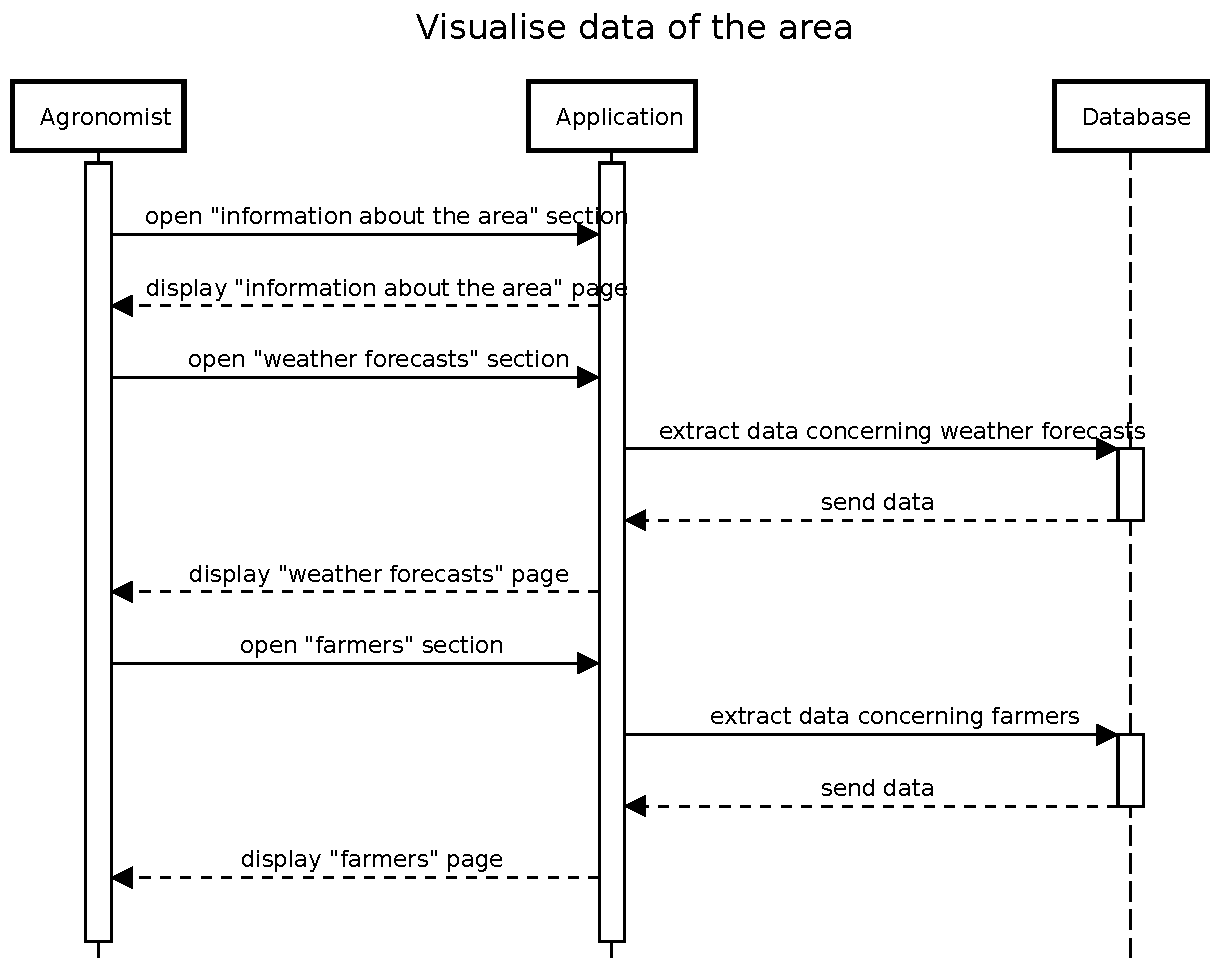
\includegraphics[scale=0.65]{Images/Sequence diagrams/Agronomist - visualise data of the area.pdf}

    \caption{Visualize data of an area - sequence diagram}
    \label{fig:fig:seq_diag_visualize_area}
\end{figure}

% USE CASE TABLE 4: ACCESS THE "DAILY PLAN" SECTION


\begin{table}[H]
    \centering
    \begin{tabular}[c]{|l|p{0.75\textwidth}|}
        \hline % ---------------------------------------------------------------------
    	\textsc{id}                 &   A.5\\
    	\hline % ---------------------------------------------------------------------
    	\textsc{Name}               &   Visualize and update a daily plan\\
    	\hline % ---------------------------------------------------------------------
    	\textsc{Actors}             &   Agronomist\\
    	\hline % ---------------------------------------------------------------------
    	\textsc{Entry conditions}   &   \begin{itemize}
                                    	    \item Agronomist has logged in
                                    	    \item At least one daily plan is present
                                        \end{itemize}\\
    	\hline % ---------------------------------------------------------------------
    	\textsc{Events flow}         &   %\footnotesize
            	                        \begin{itemize}
                                    	    \item Agronomist goes to the “Daily Plan” section, which is divided in “Visualize/Update” and “Confirm/Specify deviation from”. Agronomist selects the “Visualise/Update” section
                                    		\item The system extracts the data from the database and displays the list of daily plans for that agronomist
                                    		\item Agronomist selects a daily plan
                                    		\item The system displays all the information about that daily plan (day-month-year, farmers to be visited)
                                    		\item Agronomist clicks on the “Update” button
                                    		\item The system displays the list of farmers contained in the selected daily plan
                                    		\item Agronomist clicks on the “Remove” button near the farmer he wants to remove
                                            \item The systems displays the updated list of farmers
                                            \item Agronomist clicks on the “Add farmer” button
                                            \item The system displays the list of all the farmers for which the agronomist is responsible of and that are not already in the selected daily plan. In addition, for each farmer it is shown the list of problems encountered and the list of past and future visits (planned also by other agronomists) in a sort of compact calendar
                                            \item Agronomist selects a subset of farmers and clicks on “Add”
                                            \item The system displays the updated list of farmers
                                            \item Agronomist checks the info and clicks on “Confirm changes”

                                        \end{itemize}\\
        \hline % ---------------------------------------------------------------------
        \textsc{Exit condition}    &  The system shows a popup to notify the agronomist of the success of the operation
        \\
    	\hline % ---------------------------------------------------------------------
    	\textsc{Output}             &  \begin{itemize}
    	    \item The updated daily plan is stored in the database
    	\end{itemize}\\
    	\hline % ---------------------------------------------------------------------
    	\textsc{Exceptions}         &  \begin{itemize}
    	    \item The selected daily plan has already been confirmed and cannot be updated anymore. The system shows an error message.
    	    \item The selected daily plan is referring to the current day and cannot be updated anymore. The system shows an error message.
    	    \item Agronomist has made the wrong modifications to the daily plan. Instead of clicking “Confirm changes”, he/it clicks on “Discard changes”. The system displays the original daily plan and doesn’t store the new one in the database.    	\end{itemize}\\
    	
    	\hline % ---------------------------------------------------------------------
        
    \end{tabular}
    \caption{\label{tab:daily_plan_section_access}Visualize and update a daily plan}
\end{table}

\begin{figure}[H]
    \centering
    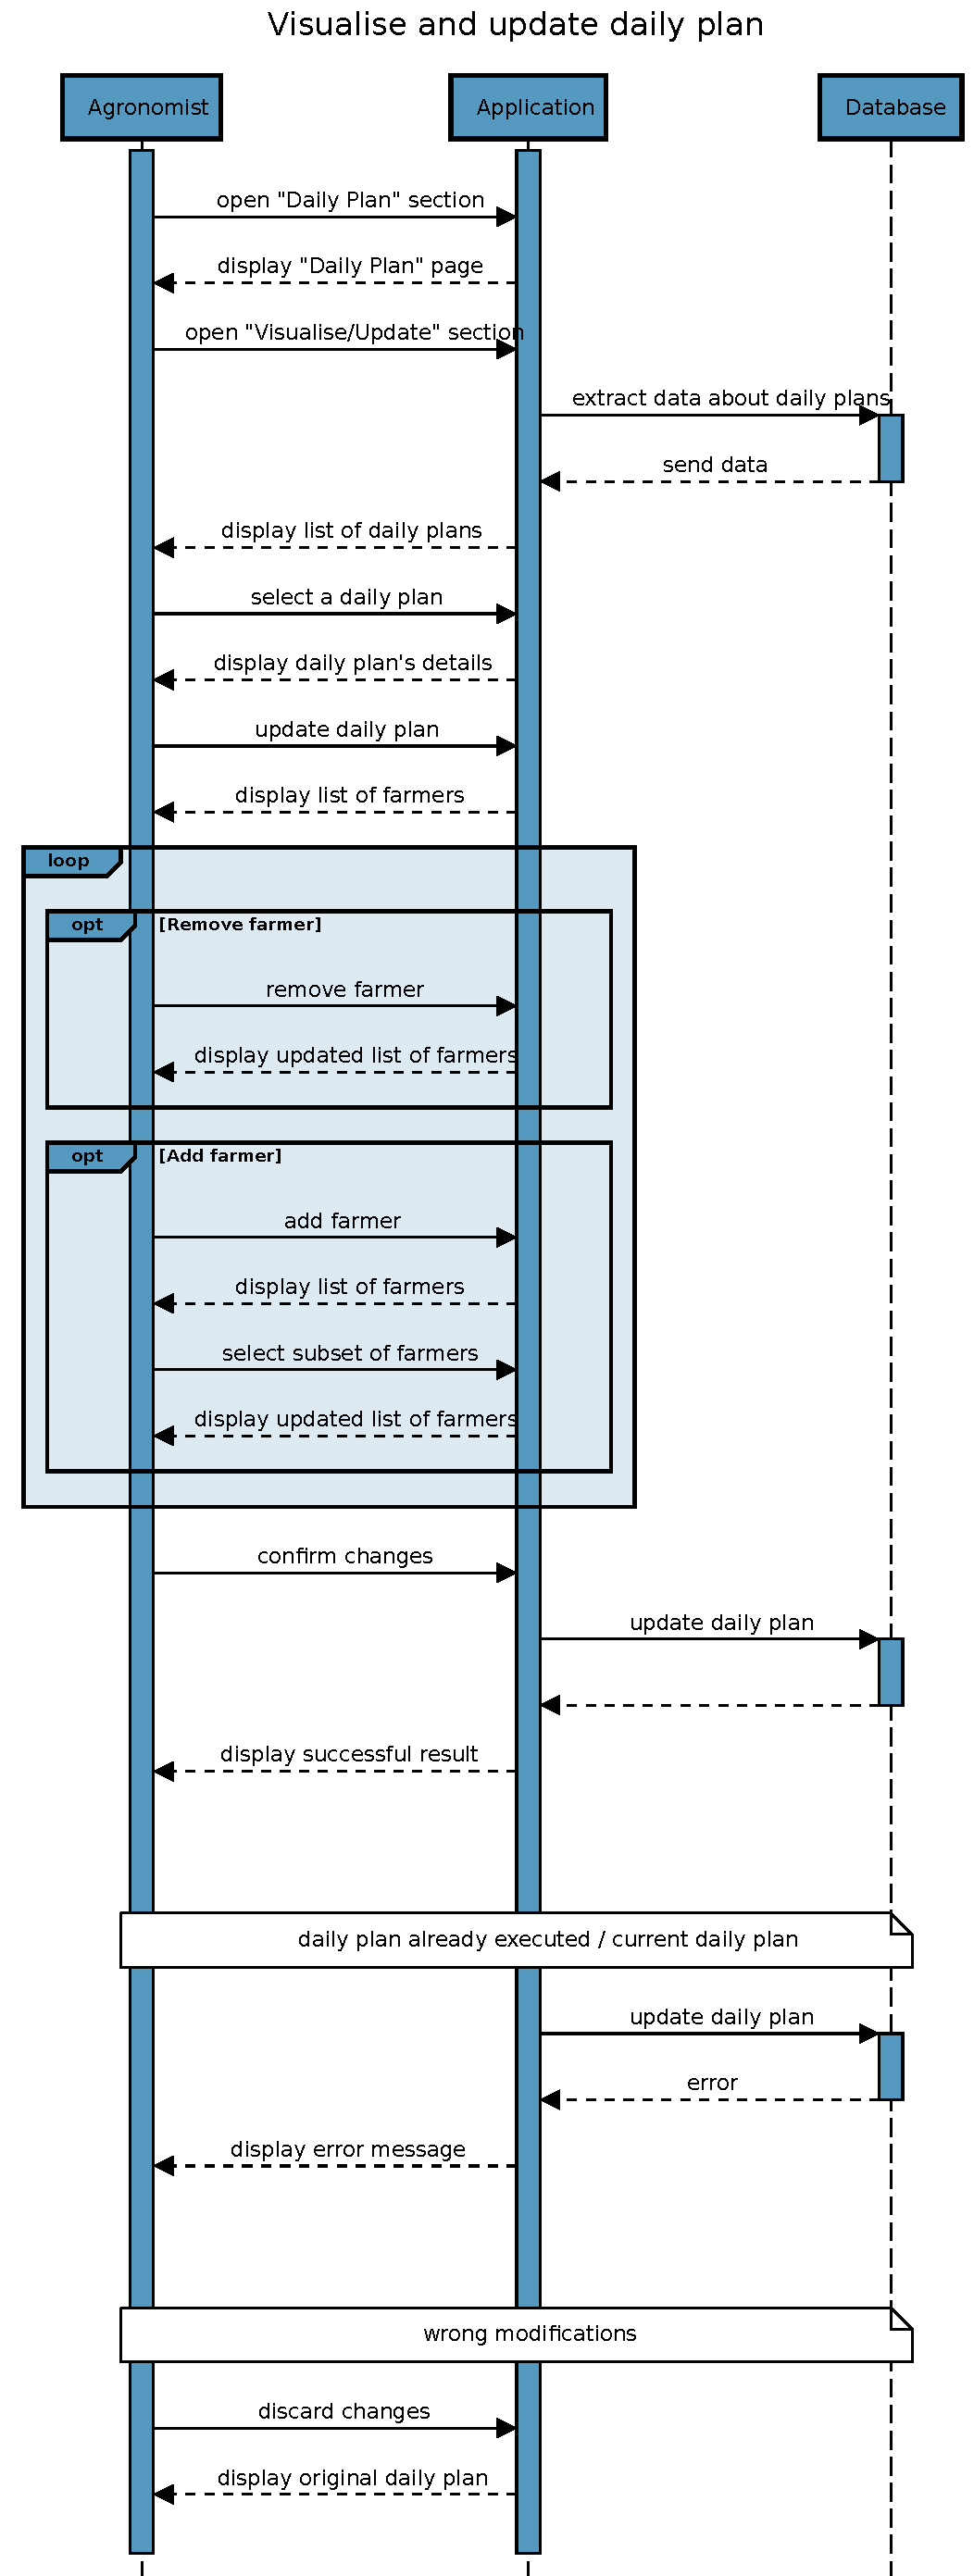
\includegraphics[scale=0.45]{Images/Sequence diagrams/Agronomist - visualise and update daily plan.pdf}

    \caption{Visualize and update a daily plan - sequence diagram}
    \label{fig:fig:seq_diag_update_daily_plan}
\end{figure}

% USE CASE TABLE 5: CONFIRM DEVIATIONS FROM DAILY PLAN


\begin{table}[H]
    \centering
    \begin{tabular}[c]{|l|p{0.75\textwidth}|}
        \hline % ---------------------------------------------------------------------
    	\textsc{id}                 &   A.6\\
    	\hline % ---------------------------------------------------------------------
    	\textsc{Name}               &   Confirm execution of daily plan\\
    	\hline % ---------------------------------------------------------------------
    	\textsc{Actor}             &   Agronomist\\
    	\hline % ---------------------------------------------------------------------
    	\textsc{Entry conditions}   &   \begin{itemize}
                                    	    \item Agronomist has logged in
                                    	    \item Agronomist has at least one daily plan
                                        \end{itemize}\\
    	\hline % ---------------------------------------------------------------------
    	\textsc{Events flow}         &   %\footnotesize
            	                        \begin{itemize}
                                    	    \item Agronomist goes to the “Daily Plan” section, which is divided in “Visualize/Update” and “Confirm/Specify deviation from”. Agronomist selects the “Confirm/Specify deviation from” section.
                                    		\item The system extracts the data from the database, displays the daily plan for the current day and enables the agronomist to select the subset of farmers which has not been visited that day
                                            \item Agronomist checks the info, selects the subset of farmers and clicks on “Continue”
                                            \item The system displays a compact summary of the info and asks for confirmation
                                            \item Agronomist checks the info and clicks on “Confirm”

                                        \end{itemize}\\
        \hline % ---------------------------------------------------------------------
        \textsc{Exit condition}    &  The system shows a popup to notify the agronomist of the success of the operation
        \\
    	\hline % ---------------------------------------------------------------------
    	\textsc{Output}             &  \begin{itemize}
    	    \item The system stores the completed daily plan in the database 
            \item The system increments by one the number of visits received by the farmers that actually have been visited
            \item The system rearranges the non-visited farmers in future daily plans

    	\end{itemize}\\
    	\hline % ---------------------------------------------------------------------
    	\textsc{Exception}         &  Agronomist has selected the wrong subset of farmers. Given the compact summary, it clicks on “Cancel”. The system displays again the daily plan and enables the agronomist to choose another subset of farmers.\\
    	
    	\hline % ---------------------------------------------------------------------
        
    \end{tabular}
    \caption{\label{tab:confirm_deviations_section}Confirm execution of daily plan}
\end{table}

\begin{figure}[H]
    \centering
    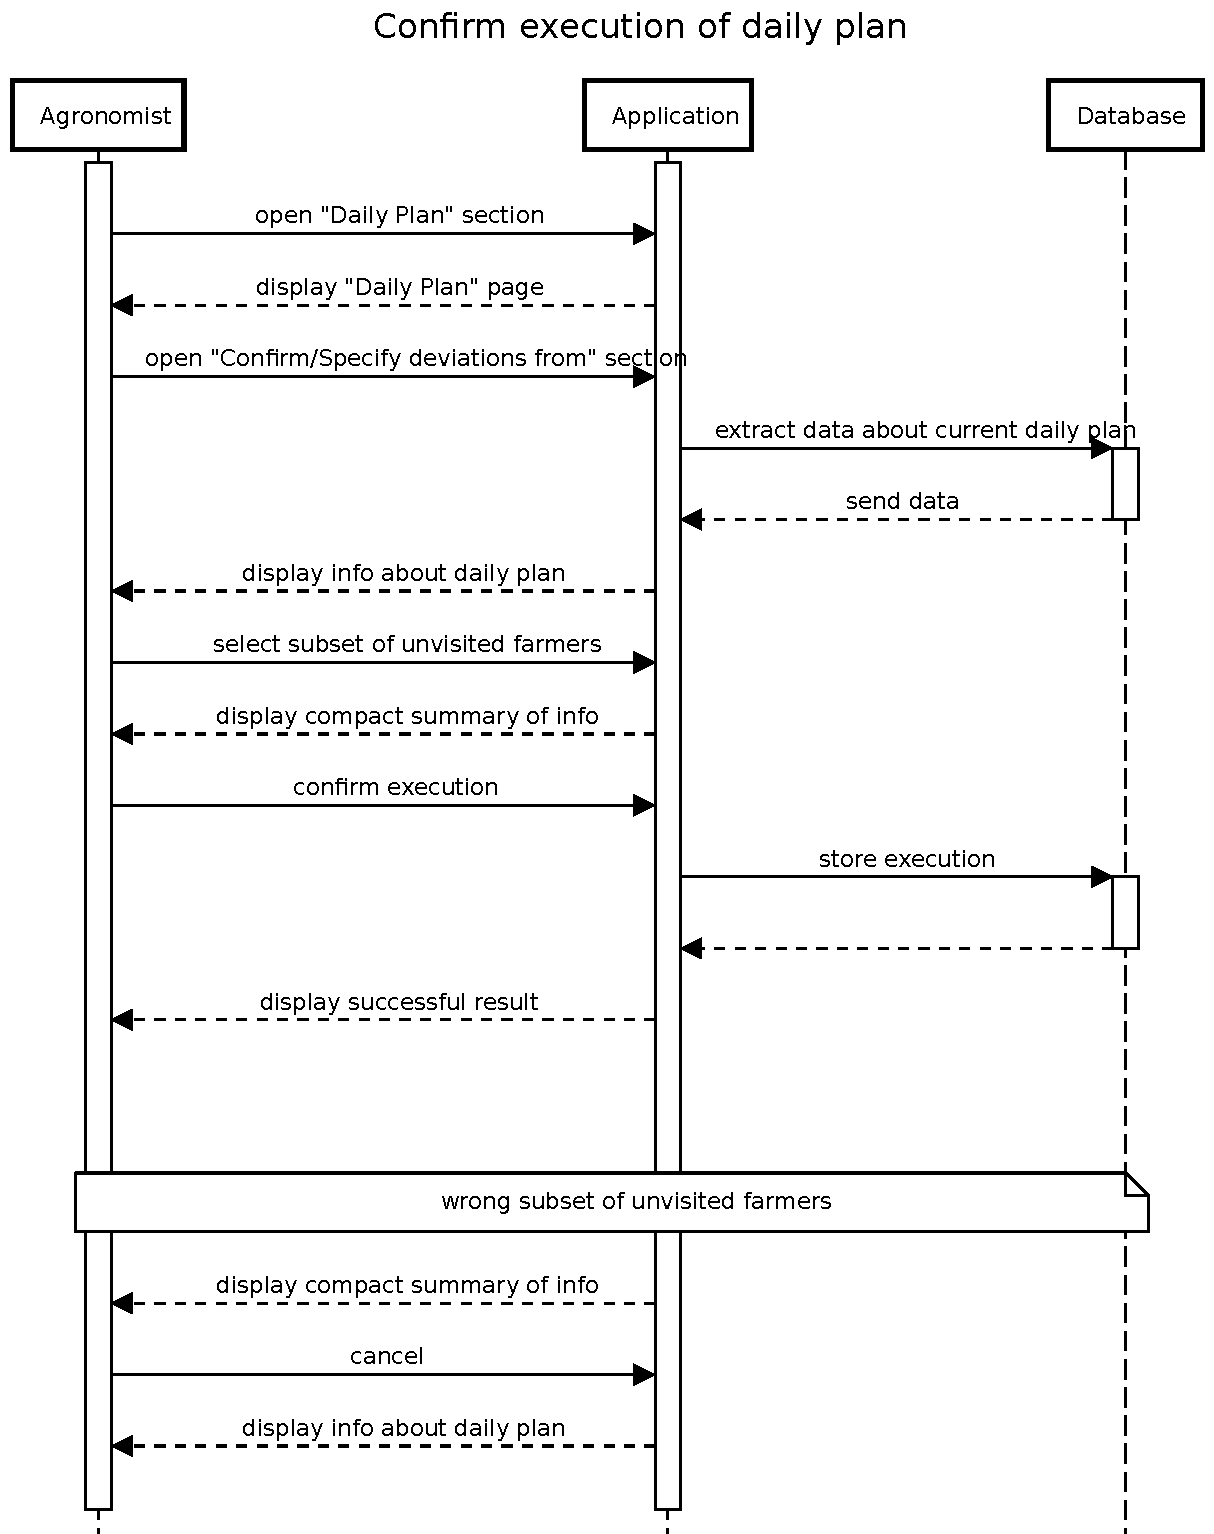
\includegraphics[scale=0.75]{Images/Sequence diagrams/Agronomist - confirm execution of daily plan.pdf}

    \caption{Confirm execution of daily plan - sequence diagram}
    \label{fig:fig:seq_diag_confirm_daily_plan}
\end{figure}

\subsubsection{User scenarios}
In this section we present a set of possible situations in 
\subsubsection{Policy maker scenarios}
\subsubsection{Farmer scenarios}

\subsubsection{Agronomist scenarios}
\subsubsection{Requirements}
\subsubsection{Traceability Matrix}

\subsection{Performance Requirements}

The system should have a good general response time, that may change depending on the specific service offered. Here are some numeric examples the system might follow:
\begin{itemize}
    \item messages and requests for help may be delivered in 5 seconds, or less;
    \item daily plans may be accessed in 7 seconds, or less;
    \item data concerning areas, with information about farmers and weather forecasts, may be given in 10 seconds, or less;
    \item registration and login operations may be confirmed in 6 seconds, or less.
\end{itemize}
It is important to notice that these numbers will also depend on the Internet connection of the users, which is assumed to be good.
\newline
\newline
The average workload of the system is expected to be very high since the user base is quite big (in the order of hundreds of thousands or even millions, considering Telangana’s population and farming prevalence) and could grow over time, if the system is extended to other states. The system should guarantee millions of operations every day, including messages, requests, access to data, etc. This could be accomplished with a good distribution of the work among the components of the system, especially during daytime. 
\newline
\newline
Since most of the operations are handled by the servers of the system, the mobile app may be lightweight, in order to be reactive and to occupy little memory on the user’s device. Also the web page should be lightweight and responsive. These software elements should take into account communication protocols unreliability.
\newline
\newline
The system interacts a lot with external services, collecting and providing data and exploiting computational analysis on such data. All the data transmission with these third party entities should be reasonably fast and scalable on the increasing number of users over time.


\subsection{Design Constraints}

\subsubsection{Standards compliance}
According to UNDP GitHub repository (ref.\cite{UNDP_GitHub}) the required platform will be compliant to DPG Standards (ref.\cite{DPGS}) that defines open-source software, open data, open AI models, open standards, and open content that adhere to privacy and other applicable best practices, do no harm by design and are of high relevance for attainment of the United Nations 2030 \href{cell:sdg}{SDGs}.

\subsubsection{Privacy constraints}
The above mentioned collection of standards \cite{DPGS} is responsible to check also privacy related requirements that have to be guaranteed. In particular it shall ensure adherence with relevant privacy, domestic, and international laws such as \href{tab:acronyms_table}{GDPR} or the ECOWAS supplementary act  in order to be accepted as a reliable software. When a user registers to the application, the privacy policy must be read and accepted, otherwise, he/she will not be able to use the service. By the fact that the platform is going to cover Telangana's territory, then STQC directorate of the Ministry of Electronics and Information Technology \cite{DPGS} data privacy standards shall be the minimum required constraints to be satsfied.


\subsubsection{Hardware limitations}

\subsection{Software System Attributes}
\subsubsection{Usability}
The system should be very easy to use, since the user base is very large and various and also comprehends many farmers. The graphical interface of both the web application and the smartphone application should help the users to identify the proper choice on the screen.
\subsubsection{Reliability}
The system should be fault tolerant in order to prevent downtime. The highest number of accesses is expected to be in the early morning (e.g., agronomists accessing the daily plan, policy makers monitoring the results) and in the late afternoon (e.g., agronomists confirming the execution of the daily plan, farmers inserting info about their production and problems).
\newline
Redundancy may be considered for a storage implementation, in order to recover from eventual data losses and to guarantee the lowest MTTR (Mean Time To Repair) possible.
\subsubsection{Availability}
The system should offer its functionalities as long as possible, with an availability of 99\% or more, so that 3.65 days of downtime per year are allowed. Some critical parts, for example the daily plan handler or the request for help platform, may have an higher availability value of 99.9\%, so that only 8.76 hours of downtime per year are allowed. 
\newline
Possible maintenance procedures in the database or in the servers may be performed using replicas or at night, in order to ensure continuity to the service.
\subsubsection{Security}
The communication between parties should be encrypted and sent along secure channels (e.g., using SSL and HTTPS protocols), in order to guarantee the protection of user’s sensitive data. 
\newline
The system should guarantee that all the operations on the database are always authorized, for example performing Role Based Access Control (RBAC), an authorization scheme that grants access rights based on the role of the user.
\subsubsection{Portability}
Since it is a Digital Public Good, the system will be compatible with the principal operating systems, either computers and mobile, and the principal web browsers. The downloadable application will be available for both Android and iOS, using for example cross platform development tools.
\subsubsection{Maintainability}
The system may be composed of scalable and reusable modules, which are easier to maintain and replace in case of failure. The source code may be commented as well as possible and the correlated documentation may be kept updated during the whole lifecycle of the system. Ordinary maintenance, for bug fixes and improvements, may be scheduled for night time, when the user traffic is minimal.
\subsubsection{Scalability}
The system should guarantee high scalability for future upgrades and expansions. For this purpose, modularity and low coupling are key aspects of the designing and developing phases.